%% =============================================================================
%%  date2027.tex -- An Exact Snoop Filter for Seamless Cache Coherence
%%
%%  Build:  pdflatex date2027.tex   (twice)
%%  Camera ready, with names and the repository URL:
%%          pdflatex "\def\CAMERAREADY{}%% =============================================================================
%%  date2027.tex -- An Exact Snoop Filter for Seamless Cache Coherence
%%
%%  Build:  pdflatex date2027.tex   (twice)
%%  Camera ready, with names and the repository URL:
%%          pdflatex "\def\CAMERAREADY{}%% =============================================================================
%%  date2027.tex -- An Exact Snoop Filter for Seamless Cache Coherence
%%
%%  Build:  pdflatex date2027.tex   (twice)
%%  Camera ready, with names and the repository URL:
%%          pdflatex "\def\CAMERAREADY{}%% =============================================================================
%%  date2027.tex -- An Exact Snoop Filter for Seamless Cache Coherence
%%
%%  Build:  pdflatex date2027.tex   (twice)
%%  Camera ready, with names and the repository URL:
%%          pdflatex "\def\CAMERAREADY{}\input{date2027}"
%%
%%  Defaults to anonymous. DATE's blind-review policy for the research track
%%  must be confirmed before submission -- the repository URL de-anonymises the
%%  work instantly, so it is behind the same toggle as the author block.
%% =============================================================================
\documentclass[conference]{IEEEtran}
\IEEEoverridecommandlockouts

\usepackage{cite}
\usepackage{amsmath,amssymb}
\usepackage{graphicx}
\usepackage{booktabs}
\usepackage{url}
\usepackage[hidelinks]{hyperref}

\ifdefined\CAMERAREADY \newif\ifanon \anonfalse \else \newif\ifanon \anontrue \fi

\begin{document}

\title{An Exact Snoop Filter for Seamless Cache Coherence in
FPGA-Based Multi-Core RISC-V}

\ifanon
  \author{\IEEEauthorblockN{Anonymous submission}}
\else
  \author{\IEEEauthorblockN{Krishna Gorai}
  \IEEEauthorblockA{Indian Institute of Technology Mandi\\
  Mandi, Himachal Pradesh, India}
  \and
  \IEEEauthorblockN{Bikram Paul}
  \IEEEauthorblockA{Indian Institute of Technology Mandi\\
  Mandi, Himachal Pradesh, India}}
\fi

\maketitle

\begin{abstract}
Attaching a private, snoop-coherent L1 data cache to an unmodified RISC-V core
is an attractive way to build FPGA multi-core systems, and a recently proposed
design does so with coherence handled entirely in hardware. We reproduce that
design in open-source RTL and measure where its time actually goes. Across four
benchmark kernels the cluster issues 1{,}048{,}821 invalidation broadcasts and
not one of them invalidates a line in another cache. Every kernel partitions its
data per processing element, so every written line is private, yet each write
still pays a cluster-wide arbitration and a handshake that waits on every other
cache. That accounts for between 6 and 33\% of a core's execution time, and on a
streaming kernel it makes the cache extension slower than having no cache at
all. We add a snoop filter that keeps an exact mirror of the caches' tag arrays
and suppresses a broadcast when no other cache holds the line or is fetching it
-- a distinction that is not cosmetic, since a mirror of committed tags alone
loses invalidations. It costs 1{,}064
LUTs and 516 flip-flops, preserves coherence under a version-monotonicity
checker, and is worth a geometric mean $1.12\times$, up to $1.22\times$ on
matrix multiplication. It also converts the streaming kernel from $0.98\times$
to $1.10\times$ against an uncached baseline. We report the frequency it costs,
and evaluate at the original design's own 60~MHz operating point.
\end{abstract}

\begin{IEEEkeywords}
RISC-V, cache coherence, snoop filter, FPGA, multi-core
\end{IEEEkeywords}

% =============================================================================
\section{Introduction}
% =============================================================================

A soft multi-core system on an FPGA gains a great deal from being able to attach
a data cache to an existing, verified RISC-V core without modifying it. The core
stays an unmodified IP block, coherence is handled in hardware, and software
needs no knowledge of either. Kamaleldin \emph{et al.}~\cite{kamaleldin2024}
propose exactly this: a private write-through L1 data cache unit (DCU) attached
through the core's ordinary memory interface, with a snooping invalidation bus
maintaining coherence across the cluster.

We built that design from scratch in open-source SystemVerilog in order to
measure it, and the measurement is the origin of this paper. The DCU exports
per-access cycle accounting, and it says that between 6 and 33\% of a core's
time is spent waiting on the coherence bus. That is a large number for a
mechanism that, on these workloads, turns out to accomplish nothing at all:
across four kernels the cluster sends 1{,}048{,}821 invalidation broadcasts and
none of them invalidates a line anywhere.

The reason is structural rather than accidental. The kernels are data-parallel
and partition their arrays per processing element, so almost every written line
is private to the core writing it. The bus has no way to know that, so every
write is announced to every cache, and the announcement is serialised: at most
one invalidation is granted per cycle, and the grant is withheld until every
other cache is ready to accept the broadcast.

Our contributions are:

\begin{itemize}
  \item A measurement of how much of this design's coherence traffic is
        necessary. On its own benchmark kernels, none of it is, and we quantify
        what that costs (Section~\ref{sec:measure}).
  \item An exact snoop filter: a structural mirror of the caches' tag arrays
        that lets the bus suppress a broadcast no cache needs. Exactness has to
        be over the right property -- a mirror of committed tags alone is
        unsound, because a cache with a refill in flight holds nothing yet and
        must still be told -- and we measure how often that distinction decides
        a coherence violation (Section~\ref{sec:filter}).
  \item An evaluation in cycles, in coherence correctness, and in
        place-and-routed FPGA cost, including the frequency the mechanism costs
        and the operating point at which it pays (Section~\ref{sec:eval}).
  \item Three mechanisms we designed, measured and rejected before this one,
        including one that was incorrect while passing every functional test it
        had (Section~\ref{sec:rejected}).
\end{itemize}

% =============================================================================
\section{Related Work}
% =============================================================================

Filtering snoops is not a new idea, and the value here is not the concept but
where the filter sits, what it is exact about, and what it is measured against.

JETTY~\cite{jetty} places a small cache-like structure between the bus and each
processor's L2, filtering snoops that would miss locally so that the energy of a
tag lookup is not spent. Its target is energy, its position is the receiving
side, and it is approximate: a small JETTY filters most useless snoops, not all.
Coarse-grain coherence tracking~\cite{cgct} and RegionScout~\cite{regionscout}
raise the granularity instead, tracking sharing over regions of hundreds or
thousands of bytes so that a region known to be unshared needs no broadcast at
all, trading precision for a much smaller structure.

Our setting inverts the cost that matters. On a snooping bus in a soft
multi-core, the expense of an unnecessary invalidation is not the energy of the
remote tag lookups but the \emph{serialisation}: one grant per cycle across the
cluster, held until every other cache is ready to accept the broadcast. The
filter therefore belongs at the source, deciding whether to arbitrate at all,
rather than at each receiver deciding whether to look. And because the design is
small -- four caches of 128 lines each -- an exact mirror is affordable, at
1{,}064 LUTs (Section~\ref{sec:eval}), which removes the need to trade precision
for size and reduces the correctness argument to a sentence. A region-based
scheme would be the right choice at a scale where an exact mirror is not
affordable; at this one it is not necessary.

The RISC-V ecosystem offers coherent fabrics at a range of scales:
TileLink~\cite{tilelink} as a coherent interconnect standard,
OpenPiton~\cite{openpiton} scaling directory coherence to many cores, and
CIFER~\cite{cifer} integrating coherent clusters in silicon. These are complete
memory systems, and adopting one means adopting its interconnect. The design
studied here occupies a deliberately different point: an extension attached to
an unmodified core through its existing memory port, which is what makes it
attractive on an FPGA and also what confines coherence to a single shared bus.
Our contribution is to that design point, not to coherent fabrics generally.

Finally, the measurement itself has a precedent worth acknowledging. JETTY's
premise is the observation that many snoops find no copy elsewhere. On the
benchmark kernels of the design studied here, \emph{no} invalidation finds a
copy elsewhere -- Section~\ref{sec:measure} establishes that, and it is the
result the rest of this paper follows from. The difference between "many" and
"all" is a property of data-parallel workloads on a private-cache cluster, and
it is what makes an exact filter worth its area here.

% =============================================================================
\section{The Design Under Study}
% =============================================================================

\begin{figure*}[t]
\centering
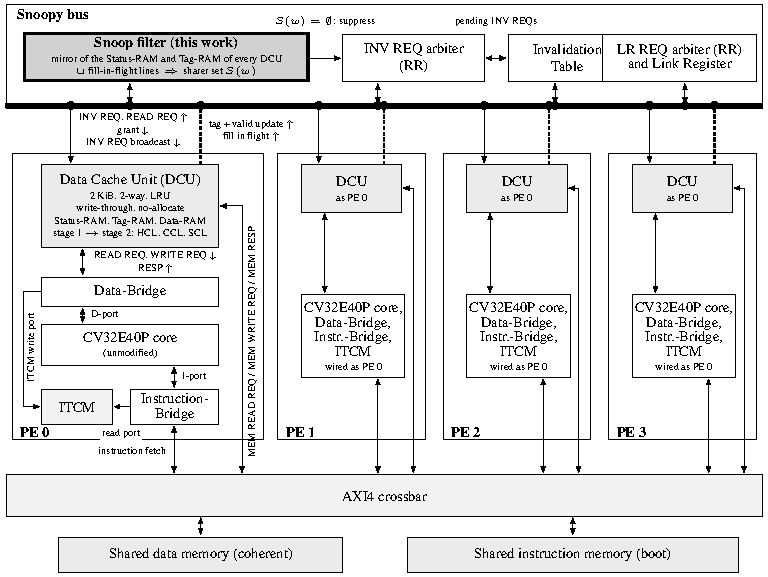
\includegraphics[width=\textwidth]{fig_arch.pdf}
\caption{The system, and what this work adds to it. Four unmodified cores sit
over their private data cache units, which reach shared memory through an AXI4
crossbar and maintain coherence through a single snoopy bus. The snoop filter
holds a mirror of every cache's tag and valid arrays, kept current by one update
port per DCU, and answers the invalidation arbiter's one question: is there
anybody to tell?}
\label{fig:arch}
\end{figure*}

The DCU is a private, write-through, no-allocate L1 data cache sitting between
an in-order RISC-V core and the memory system. Because writes go through to
memory, shared memory always holds the current value and no dirty-line writeback
or ownership state is needed. Coherence is maintained by an invalidation bus:
a core write reaches the bus as an invalidation request, and on grant the
address is broadcast to every other DCU, which drops any matching line.

Two properties of that bus matter here. Plain read requests are not arbitrated
against each other -- multiple readers proceed in the same cycle, which is the
multiple-readers half of the MRSW invariant -- but a read is withheld while
another core has an invalidation outstanding for the same line, which is the
single-writer half. Invalidations \emph{are} arbitrated: at most one is granted
per cycle across the cluster, and the grant is held back until every other DCU
can accept the broadcast, so that no invalidation is ever lost.

Fig.~\ref{fig:arch} shows the system and where the filter sits in it.
Our reproduction targets the stated configuration: four processing elements,
each an unmodified CV32E40P with a private 2\,KiB two-way DCU of 16-byte lines,
meeting shared memories through an AXI4 crossbar. A non-coherent baseline is
built from the same sources with one parameter changed, so any comparison
between them is attributable to the cache sub-system alone.

% =============================================================================
\section{Where the Time Goes}
\label{sec:measure}
% =============================================================================

\subsection{The coherence bus is a large fraction of runtime}

The DCU separates a core access into the places it can wait. One of those is
stage~1 waiting for a snoopy-bus grant. Fig.~\ref{fig:stall} gives that bucket
as a fraction of the cycles a core spent with an access in the DCU at all,
for each kernel at three memory latencies.

\begin{figure}[t]
\centering
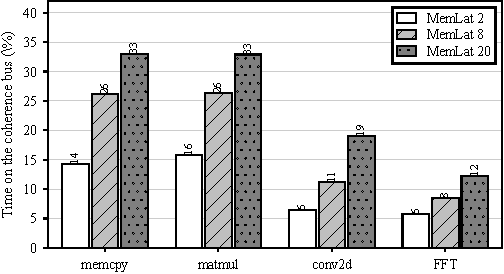
\includegraphics[width=\columnwidth]{fig_stall.pdf}
\caption{Time each core spends waiting for a snoopy-bus grant, as a percentage
of the cycles it had an access in the DCU. Table~\ref{tab:invuse} shows that
none of the traffic it is waiting for is necessary.}
\label{fig:stall}
\end{figure}

Between a twentieth and a third of a core's time goes to arbitrating for a
resource that grants one request per cycle across the whole cluster. The share
grows with memory latency, because each grant is held longer.

\subsection{It is not readers waiting on writers}

The obvious reading of Fig.~\ref{fig:stall} is contention between readers and
writers -- the single-writer screening doing its job. We instrumented the bus to
count it, and across all four kernels a read is \emph{never} withheld: not once.
Whatever the stall is, it is not the MRSW screening.

By elimination it is the invalidations, which are the only arbitrated traffic
left.

\subsection{None of the invalidations are necessary}

Each DCU therefore counts the broadcasts it receives and how many find a line to
clear. Table~\ref{tab:invuse} gives the result.

\begin{table}[t]
\caption{Invalidation broadcasts received across the cluster, and how many
invalidated a line. The last row is a control.}
\label{tab:invuse}
\centering
\begin{tabular}{@{}lrrr@{}}
\toprule
Workload & Broadcasts & Useful & \% \\
\midrule
matmul ($64^2$)      & 823{,}338 & 0 & 0.00 \\
conv2d ($64^2$)      & 139{,}182 & 0 & 0.00 \\
FFT ($N{=}256$)      &  61{,}683 & 0 & 0.00 \\
memcpy (16\,KiB)     &  24{,}618 & 0 & 0.00 \\
\midrule
sharing testbench    &       921 & 345 & 37.46 \\
\bottomrule
\end{tabular}
\end{table}

Over a million broadcasts, none of which invalidated anything. Each one paid a
cluster-wide arbitration and a four-way handshake to inform nobody of anything.

A result this uniform deserves suspicion of the instrument rather than of the
design, so the counter is controlled. Our coherence testbench shares
deliberately, with a producer/consumer ping-pong and a randomised four-core
stress over a small window; on that workload the same counter reports 345 useful
broadcasts of 921. The counter can see a useful invalidation. The zeroes are a
property of the workloads.

They are a property worth stating plainly: these kernels are data-parallel and
partition their data per core, so essentially every written line is private.
That is not a weakness of the benchmark selection, because these are the kernels
the original evaluation itself uses.

% =============================================================================
\section{An Exact Snoop Filter}
\label{sec:filter}
% =============================================================================

\subsection{Structure}

The bus needs to answer one question before granting an invalidation: is there
another cache that has to hear it? A mirror of the caches' tag and valid arrays
answers it, held in the bus and updated by the same two events that change the
caches themselves -- a refill installs a tag into a way, an invalidation clears
one. Each DCU exports those events on a small port driven from the same signals
that write its own arrays.

Exactness is therefore structural rather than argued. The mirror is written from
the same signals, on the same clock edge, under the same conditions as the state
it mirrors, so it cannot drift from it.

We rejected a hashed filter deliberately. A Bloom-style structure may only ever
over-approximate: claiming a line is held when it is not costs a redundant
broadcast and is safe, while the converse loses an invalidation and breaks
coherence. Insert-only hashed filters are safe but saturate, and matmul touches
far more lines than an affordable bitmap has bits; removing from one requires
knowing when a line leaves a cache, which is exactly the information a mirror
already has.

\subsection{Exact about the wrong property}
\label{sec:fill}

A mirror of the tag arrays is exact about which lines each cache \emph{holds},
and that turns out not to be the property the bus needs. A DCU between issuing
its memory read and refilling the victim way holds nothing for the line it is
fetching, so it does not appear in the mirror -- and it is precisely the cache
that must receive the invalidation, because receiving one in that window is what
cancels its refill. Suppress the broadcast and it installs a line that was
invalidated while in flight.

The property is residency \emph{or imminent residency}. Each DCU therefore
exports its refill window alongside its mirror updates, and the filter answers
over the union. The window opens when the cache issues the fetch and closes on
the cycle the refill lands, which is the same cycle the mirror learns the tag:
the two halves abut exactly, so the line is covered in every cycle by one or the
other.

This is not a defensive addition. Counting the granted invalidations for which
no other cache held the line but one was fetching it -- each one a broadcast a
committed-tag mirror would have wrongly suppressed -- our coherence testbench
reports 20 of 2{,}241 over ten randomised interleavings, and at least one in
every one of the ten. The window is narrow enough that the design passed 3{,}139
checks before the counter existed, which is how a race of this shape usually
survives a test suite.

\subsection{Why suppression is safe}

When the answer is that no other cache holds the line or is fetching it, a
broadcast could clear nothing anywhere, and not sending it is unobservable. That
is the whole argument, and it is short because the structure is exact. A
conservative filter would need an argument about the direction of its error;
this one needs only that it asks about the right state.

Everything else is untouched. Invalidations that \emph{are} needed are still
arbitrated, broadcast and acknowledged exactly as before; the single-writer
screening on reads is unchanged; and the write-through lock that stops a remote
read fetching a pre-write value is unchanged, because it protects against a
value in memory rather than against a cached copy.

\subsection{Implementation}

The mirror is one array per (core, way) pair, each with a single write port and
a single read port, addressed by set index -- eight arrays at the geometry
studied here. Tags are held outside any reset, since a tag is only compared when
its valid bit says it means something, which lets them map to distributed RAM.
Valid bits stay in flip-flops, where they can be reset and read eight at a time,
at 512 bits rather than 11{,}264. This is the same division the DCU makes
internally for the same reason.

That structure matters more than it might appear: a first implementation held
tags and valid bits together under an asynchronous reset and read them
combinationally, which Vivado mapped entirely to flip-flops -- 11{,}776 of them,
and 3{,}202 LUTs, against 512 and 408 for the structure above.

% =============================================================================
\section{Evaluation}
\label{sec:eval}
% =============================================================================

\subsection{Cycles}

\begin{figure*}[t]
\centering
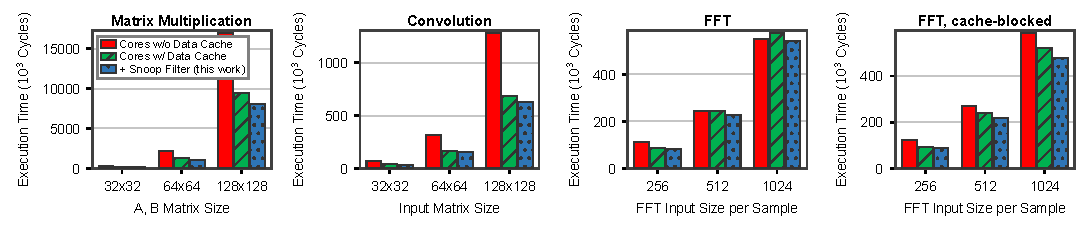
\includegraphics[width=\textwidth]{fig_exec.pdf}
\caption{Execution time of the three benchmark kernels against problem size,
without a data cache, with one, and with the snoop filter of this work. The
axes are those of the original's own execution-time figure, so the first two
bars of each cluster are directly comparable with it. Matrix multiplication and
convolution reproduce the reduction it reports; FFT does not, and the reason is
capacity rather than coherence -- see the text.}
\label{fig:exec}
\end{figure*}

Fig.~\ref{fig:exec} places the extension on the original's own axes: execution
time per kernel against problem size, uncached against cached, with our filter
added as a third bar the original has no counterpart to.

Two of the three reproduce it: matrix multiplication by 38.4 to 44.0\% and
convolution by 46 to 48\%, against the ${\approx}40\%$ the original reports for
both. Neither decays with problem size, and that is not luck. What must stay resident is not the data set but the \emph{reuse
footprint}, the bytes a core revisits before moving on -- one row of $B$ for
matrix multiplication, $4N$ bytes or 512\,B at $N{=}128$, and the three-row
sliding window for convolution, $12N$ bytes or 1536\,B. Both fit a 2\,KiB DCU
throughout, so the benefit does not move.

FFT is where that stops holding. The original reports a uniform
${\approx}23\%$; we match it at $N{=}256$, at 24.8\%, but the benefit falls to
0.4\% at 512 and turns negative at 1024, where the cache makes the kernel
\emph{slower} than having none. The footprint argument predicts exactly this:
FFT revisits $N$ complex points across its stages, $8N$ bytes, which is 2\,KiB
at $N{=}256$ and 8\,KiB at $N{=}1024$. Only the first fits.

That the cause is capacity and not conflict can be shown rather than asserted,
by moving one variable at a time. At $N{=}512$, doubling associativity at the
same 2\,KiB recovers 3.8\%; quadrupling capacity at the same associativity
recovers 24.5\%, and 16\,KiB recovers nothing beyond 8\,KiB. Saturation once the
footprint fits is the signature of a capacity limit, not a conflict one. Given a
DCU that holds the footprint, FFT then reproduces the original at every size --
24.8, 24.8 and 24.5\% at 8\,KiB. At the 2\,KiB its text states, it does not. We
read that as a configuration discrepancy rather than a contradiction: its result
implies a cache larger than the one specified, or a smaller working set, and the
published description does not let a reader tell which.

None of it weakens the filter, which is orthogonal: the filter removes coherence
traffic, not misses. It is worth roughly 50\% throughout on the first two
kernels, and at $N{=}1024$ it is what carries FFT back from $-4.3\%$ to parity.

%% The per-kernel speedup table was folded into the paragraph below. Three of
%% its four rows duplicated bars now in Fig. \ref{fig:exec}; what it uniquely
%% carried -- memcpy, and the oracle column -- is two sentences, and the page
%% limit was worth more than the fourth restatement of the same four numbers.

Against the unfiltered design the filter is worth $1.222\times$ on matrix
multiplication, $1.123\times$ on memcpy, $1.089\times$ on convolution and
$1.061\times$ on FFT: a geometric mean of $1.122\times$. The useful comparison
is not that mean but an oracle that suppresses every broadcast unconditionally,
which is sound to simulate only because Table~\ref{tab:invuse} says none are
needed, and which bounds what any filter could return.

%% fig_result removed to make room for fig_exec, which supersedes it: its panel
%% (a) plotted what the extension is worth against no cache, which fig_exec now
%% does for three kernels at three sizes rather than one size each. Its panel
%% (b), the snoop-stall reduction, survives as the numbers in the paragraph
%% below -- conv2d 20,848 to 109, memcpy 7,168 to 1 -- so no evidence is lost
%% with it. paper/fig_result.pdf is still generated by scripts/plot_date.py if
%% a venue with a looser page limit wants it back.

The filter reaches the oracle on every kernel, cycle for cycle. That is what an
exact structure should do on workloads with no sharing: it suppresses precisely
the broadcasts the oracle does, for a provable reason rather than an assumed
one.

The snoop-stall bucket confirms the mechanism rather than merely the outcome.
On conv2d it falls from 20{,}848 cycles to 109; on memcpy, from 7{,}168 to 1.
FFT is the exception and falls only from 6{,}521 to 2{,}955, because
load-reserved and store-conditional still pass the second arbiter whatever the
broadcasts do -- a residual cost no filter can remove.

\subsection{The extension stops being harmful}

The reproduction's most awkward finding was that on memcpy at low memory
latency, the cache extension is \emph{slower} than having no cache at all:
$0.975\times$ the non-coherent baseline. With the filter it runs at
$1.095\times$. The pathology is not intrinsic to attaching a coherent cache; it
is the cost of announcing private writes to a cluster that does not care.

\subsection{Coherence}

The four kernels never exercise the filter's must-broadcast path, so they cannot
establish that it is safe. Our coherence testbench does: it shares deliberately,
and roughly half of its invalidations are useful. With the filter enabled it
passes 3{,}112 checks, including a version-monotonicity invariant -- a core that
has observed version $k$ of a location may never afterwards observe a version
below $k$, which is exactly what a lost invalidation causes -- and a final
quiesce in which every core re-reads the whole window so that any line left
stale in any cache is caught against memory. The filter suppressed 282 of 921
broadcasts and delivered every one that mattered.

\subsection{FPGA cost}

Both configurations were implemented on a Zynq UltraScale+ XCZU7EV in a
non-project Vivado 2025.1 flow.

\input{tab_hier}

Table~\ref{tab:fpga} gives the breakdown. The filter costs 1{,}064 LUTs and
516 flip-flops over the unfiltered design, under 4\% of it, and no block RAM or
DSP at all. Both configurations meet every constraint with no failing endpoints,
at $+1.199$~ns and $+1.265$~ns of slack respectively -- so at this operating
point the filter costs essentially no slack, 66~ps on a 16.667~ns period.

Both figures come from one source tree with one parameter changed, implemented
in the same batch, which is the only way a slack comparison on this design means
anything: an earlier pair of runs weeks apart put the same two configurations at
$+4.307$ and $+2.597$~ns, a 1.7~ns spread in the opposite direction, from
netlists differing by fourteen LUTs. Place-and-route outcomes move by more than
the effect being measured, so we quote slack only within a batch and never
across one.

Two things in the breakdown are worth drawing out. Half of the filter's 408
LUTs are distributed RAM holding the mirror, and its 512 flip-flops are exactly
the valid bits, four cores by 64 sets by two ways: the structure went in as
intended, with tags in memory and only the resettable state in registers. And
within the DCU the controller outweighs the storage, 2{,}802 LUTs against
1{,}677 for the tag array and 1{,}285 for the data array, because at 2\,KiB the
arrays are nearly free and the coherence logic is not.

\subsection{The frequency it costs}

It does cost frequency, and the paper would be misleading without saying so. At
a 75~MHz target the reference meets timing with $+1.327$~ns of slack and the
filtered design does not, at $-2.586$~ns. The critical path is 86\% routing and
runs from a DCU's registered request address across the die; the filter
lengthens it because the decision to broadcast is a cluster-spanning
combinational path, and it does so however the mirror is built. Making the
mirror smaller did not help: the flip-flop version above is four times the area
and closes \emph{better}, at $-0.423$~ns.

We therefore evaluate at 60~MHz, which both configurations meet comfortably, and
which is the frequency the original design itself runs at rather than one chosen
for convenience. At a fixed 60~MHz clock the filter's $1.122\times$ in cycles is
a $1.122\times$ in wall time. Clocked freely, the reference reaches a higher
frequency and the advantage narrows.

We deliberately do not report a maximum-frequency comparison from the 60~MHz
builds. Measured at a constraint that is already met, that figure records where
the tool stopped optimising rather than what the design can do: at 60~MHz it
favours the filtered design by 9.8~MHz, and at 75~MHz it favours the reference
by 20.5~MHz.

% =============================================================================
\section{What Did Not Work}
\label{sec:rejected}
% =============================================================================

Three mechanisms preceded this one. We report them because each was rejected by
a measurement that also sharpened the eventual design.

\textbf{A streaming mode} that would skip allocation and read at word
granularity for phases with no reuse. The non-coherent baseline already is such
a mode, and bounds it: on memcpy it beats the cache at a memory latency of two
by 2.5\% and loses by better than two to one at eight and twenty, because a line
fill amortises one memory latency across four words.

\textbf{A hit-speculative bypass}, in which a read presumes it will hit and
takes no bus transaction, and only a miss arbitrates. It was both useless and
incorrect. Useless because plain reads were never arbitrated in the first place,
so there was no cost to remove -- it measured slower. Incorrect because the
screening it removed is not about allocation but is the single-writer half of
MRSW: a read that hits a resident line while a remote invalidation for that line
is outstanding returns stale data. It passed all eleven functional checks of the
benchmark harness, which is the point worth reporting: the race window is narrow
and a green test said nothing about it.

\textbf{Two structural fixes to the mirror}, described in
Section~\ref{sec:eval}: neither the register count nor the storage type was the
cause of the frequency loss.

\textbf{Directed invalidation}, the obvious next step, which does not pay. The
mirror knows not merely \emph{whether} another cache holds the line but
\emph{which} ones do, so the bus can invalidate exactly those and hold the grant
on only those: an exact multicast with a partial barrier. Only an exact filter
may do this, since under multicast a missing sharer bit loses an invalidation
rather than costing a redundant broadcast. Measured on a halo-exchange stencil
whose band boundaries give a sharer set of exactly one of three, it behaves
perfectly -- 168 invalidations delivered, all 168 useful, against suppression's
504, with the residual stall down elevenfold -- and is worth 0.1 to 0.3\% at
every memory latency tried. Exact suppression has already removed the traffic
that caused the serialisation, and the remainder is irreducible: somebody does
have to be told, and the writer does have to wait. Once the filter is exact, the
residue is not worth steering.

% =============================================================================
\section{Threats to Validity}
% =============================================================================

The central measurement is that none of the invalidation traffic is useful, and
that is a property of workloads as much as of the design. Data-parallel kernels
that partition per core have almost nothing to share. We claim only what we
measured: on the kernels the original evaluation itself uses, this design's
coherence traffic is entirely avoidable. The halo-exchange stencil of
Section~\ref{sec:rejected} is the case with genuine sharing, and the filter is
still worth $1.11\times$ there at a memory latency of twenty, because the
interior of each band is private even when its boundary is not. Our coherence
testbench, at roughly half its invalidations useful, is the extreme in the other
direction.

The evaluation is in cycles from RTL simulation and in post-place-and-route
resource and timing figures; no bitstream has been run on hardware. The original
targets a Virtex UltraScale+ XCVU9P and this work an XCZU7EV, so absolute
figures are directional rather than a like-for-like comparison.

Power is not reported: Vivado's vectorless estimate models this design as idle,
because it cannot evaluate the cores' clock-gate enables.

% =============================================================================
\section{Conclusion}
% =============================================================================

A seamless coherent cache extension for soft RISC-V multicores spends between 6
and 33\% of each core's time on a coherence protocol that, on its own benchmark
kernels, accomplishes nothing: over a million invalidation broadcasts, none of
which invalidate anything. An exact mirror of the caches' tag arrays lets the
bus suppress those broadcasts for 1{,}064 LUTs and 516 flip-flops, preserving
coherence structurally rather than by argument, and is worth a geometric mean
$1.122\times$ at a fixed 60~MHz clock. It also removes the case in which the
extension was slower than having no cache at all. The mechanism costs
frequency, and we report where that matters.

\ifanon
\else
The design, the measurements and the scripts that regenerate every table are
available at \url{https://github.com/Krishna-Gorai/riscv-cache-extension}.
\fi

\begin{thebibliography}{1}
\bibitem{kamaleldin2024}
A.~Kamaleldin, M.~Nickel, S.~Wu and D.~G\"ohringer,
``Seamless Cache Extension for FPGA-based Multi-Core RISC-V SoC,''
in \emph{Proc. IEEE 37th Int. System-on-Chip Conf. (SOCC)}, 2024.

\bibitem{jetty}
A.~Moshovos, G.~Memik, B.~Falsafi and A.~Choudhary,
``JETTY: Filtering Snoops for Reduced Energy Consumption in SMP Servers,''
in \emph{Proc. 7th Int. Symp. High-Performance Computer Architecture (HPCA)},
2001.

\bibitem{cgct}
J.~F.~Cantin, M.~H.~Lipasti and J.~E.~Smith,
``Improving Multiprocessor Performance with Coarse-Grain Coherence Tracking,''
in \emph{Proc. 32nd Int. Symp. Computer Architecture (ISCA)}, 2005, pp.
246--257.

\bibitem{regionscout}
A.~Moshovos,
``RegionScout: Exploiting Coarse Grain Sharing in Snoop-Based Coherence,''
in \emph{Proc. 32nd Int. Symp. Computer Architecture (ISCA)}, 2005, pp.
234--245.

\bibitem{tilelink}
W.~Terpstra,
``TileLink: A Free and Open-Source, High-Performance Scalable Cache-Coherent
Fabric Designed for RISC-V,'' in \emph{RISC-V Workshop}, 2017.

\bibitem{openpiton}
J.~Balkind \emph{et al.},
``OpenPiton+Ariane: The First Open-Source, SMP Linux-booting RISC-V System
Scaling from One to Many Cores,'' in \emph{Workshop on Computer Architecture
Research with RISC-V (CARRV)}, 2019.

\bibitem{cifer}
A.~Li \emph{et al.},
``CIFER: A Cache-Coherent 12nm 16mm$^2$ SoC with Four 64-Bit RISC-V Application
Cores, 18 32-Bit RISC-V Compute Cores, and a 1541 LUT6/mm$^2$ Synthesizable
eFPGA,'' in \emph{IEEE Int. Solid-State Circuits Conf. (ISSCC)}, 2023.
\end{thebibliography}

\end{document}
"
%%
%%  Defaults to anonymous. DATE's blind-review policy for the research track
%%  must be confirmed before submission -- the repository URL de-anonymises the
%%  work instantly, so it is behind the same toggle as the author block.
%% =============================================================================
\documentclass[conference]{IEEEtran}
\IEEEoverridecommandlockouts

\usepackage{cite}
\usepackage{amsmath,amssymb}
\usepackage{graphicx}
\usepackage{booktabs}
\usepackage{url}
\usepackage[hidelinks]{hyperref}

\ifdefined\CAMERAREADY \newif\ifanon \anonfalse \else \newif\ifanon \anontrue \fi

\begin{document}

\title{An Exact Snoop Filter for Seamless Cache Coherence in
FPGA-Based Multi-Core RISC-V}

\ifanon
  \author{\IEEEauthorblockN{Anonymous submission}}
\else
  \author{\IEEEauthorblockN{Krishna Gorai}
  \IEEEauthorblockA{Indian Institute of Technology Mandi\\
  Mandi, Himachal Pradesh, India}
  \and
  \IEEEauthorblockN{Bikram Paul}
  \IEEEauthorblockA{Indian Institute of Technology Mandi\\
  Mandi, Himachal Pradesh, India}}
\fi

\maketitle

\begin{abstract}
Attaching a private, snoop-coherent L1 data cache to an unmodified RISC-V core
is an attractive way to build FPGA multi-core systems, and a recently proposed
design does so with coherence handled entirely in hardware. We reproduce that
design in open-source RTL and measure where its time actually goes. Across four
benchmark kernels the cluster issues 1{,}048{,}821 invalidation broadcasts and
not one of them invalidates a line in another cache. Every kernel partitions its
data per processing element, so every written line is private, yet each write
still pays a cluster-wide arbitration and a handshake that waits on every other
cache. That accounts for between 6 and 33\% of a core's execution time, and on a
streaming kernel it makes the cache extension slower than having no cache at
all. We add a snoop filter that keeps an exact mirror of the caches' tag arrays
and suppresses a broadcast when no other cache holds the line or is fetching it
-- a distinction that is not cosmetic, since a mirror of committed tags alone
loses invalidations. It costs 1{,}064
LUTs and 516 flip-flops, preserves coherence under a version-monotonicity
checker, and is worth a geometric mean $1.12\times$, up to $1.22\times$ on
matrix multiplication. It also converts the streaming kernel from $0.98\times$
to $1.10\times$ against an uncached baseline. We report the frequency it costs,
and evaluate at the original design's own 60~MHz operating point.
\end{abstract}

\begin{IEEEkeywords}
RISC-V, cache coherence, snoop filter, FPGA, multi-core
\end{IEEEkeywords}

% =============================================================================
\section{Introduction}
% =============================================================================

A soft multi-core system on an FPGA gains a great deal from being able to attach
a data cache to an existing, verified RISC-V core without modifying it. The core
stays an unmodified IP block, coherence is handled in hardware, and software
needs no knowledge of either. Kamaleldin \emph{et al.}~\cite{kamaleldin2024}
propose exactly this: a private write-through L1 data cache unit (DCU) attached
through the core's ordinary memory interface, with a snooping invalidation bus
maintaining coherence across the cluster.

We built that design from scratch in open-source SystemVerilog in order to
measure it, and the measurement is the origin of this paper. The DCU exports
per-access cycle accounting, and it says that between 6 and 33\% of a core's
time is spent waiting on the coherence bus. That is a large number for a
mechanism that, on these workloads, turns out to accomplish nothing at all:
across four kernels the cluster sends 1{,}048{,}821 invalidation broadcasts and
none of them invalidates a line anywhere.

The reason is structural rather than accidental. The kernels are data-parallel
and partition their arrays per processing element, so almost every written line
is private to the core writing it. The bus has no way to know that, so every
write is announced to every cache, and the announcement is serialised: at most
one invalidation is granted per cycle, and the grant is withheld until every
other cache is ready to accept the broadcast.

Our contributions are:

\begin{itemize}
  \item A measurement of how much of this design's coherence traffic is
        necessary. On its own benchmark kernels, none of it is, and we quantify
        what that costs (Section~\ref{sec:measure}).
  \item An exact snoop filter: a structural mirror of the caches' tag arrays
        that lets the bus suppress a broadcast no cache needs. Exactness has to
        be over the right property -- a mirror of committed tags alone is
        unsound, because a cache with a refill in flight holds nothing yet and
        must still be told -- and we measure how often that distinction decides
        a coherence violation (Section~\ref{sec:filter}).
  \item An evaluation in cycles, in coherence correctness, and in
        place-and-routed FPGA cost, including the frequency the mechanism costs
        and the operating point at which it pays (Section~\ref{sec:eval}).
  \item Three mechanisms we designed, measured and rejected before this one,
        including one that was incorrect while passing every functional test it
        had (Section~\ref{sec:rejected}).
\end{itemize}

% =============================================================================
\section{Related Work}
% =============================================================================

Filtering snoops is not a new idea, and the value here is not the concept but
where the filter sits, what it is exact about, and what it is measured against.

JETTY~\cite{jetty} places a small cache-like structure between the bus and each
processor's L2, filtering snoops that would miss locally so that the energy of a
tag lookup is not spent. Its target is energy, its position is the receiving
side, and it is approximate: a small JETTY filters most useless snoops, not all.
Coarse-grain coherence tracking~\cite{cgct} and RegionScout~\cite{regionscout}
raise the granularity instead, tracking sharing over regions of hundreds or
thousands of bytes so that a region known to be unshared needs no broadcast at
all, trading precision for a much smaller structure.

Our setting inverts the cost that matters. On a snooping bus in a soft
multi-core, the expense of an unnecessary invalidation is not the energy of the
remote tag lookups but the \emph{serialisation}: one grant per cycle across the
cluster, held until every other cache is ready to accept the broadcast. The
filter therefore belongs at the source, deciding whether to arbitrate at all,
rather than at each receiver deciding whether to look. And because the design is
small -- four caches of 128 lines each -- an exact mirror is affordable, at
1{,}064 LUTs (Section~\ref{sec:eval}), which removes the need to trade precision
for size and reduces the correctness argument to a sentence. A region-based
scheme would be the right choice at a scale where an exact mirror is not
affordable; at this one it is not necessary.

The RISC-V ecosystem offers coherent fabrics at a range of scales:
TileLink~\cite{tilelink} as a coherent interconnect standard,
OpenPiton~\cite{openpiton} scaling directory coherence to many cores, and
CIFER~\cite{cifer} integrating coherent clusters in silicon. These are complete
memory systems, and adopting one means adopting its interconnect. The design
studied here occupies a deliberately different point: an extension attached to
an unmodified core through its existing memory port, which is what makes it
attractive on an FPGA and also what confines coherence to a single shared bus.
Our contribution is to that design point, not to coherent fabrics generally.

Finally, the measurement itself has a precedent worth acknowledging. JETTY's
premise is the observation that many snoops find no copy elsewhere. On the
benchmark kernels of the design studied here, \emph{no} invalidation finds a
copy elsewhere -- Section~\ref{sec:measure} establishes that, and it is the
result the rest of this paper follows from. The difference between "many" and
"all" is a property of data-parallel workloads on a private-cache cluster, and
it is what makes an exact filter worth its area here.

% =============================================================================
\section{The Design Under Study}
% =============================================================================

\begin{figure*}[t]
\centering
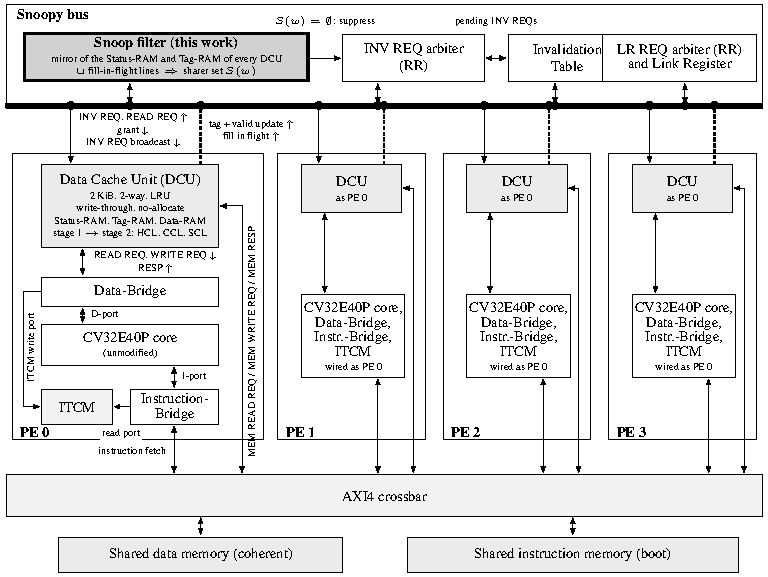
\includegraphics[width=\textwidth]{fig_arch.pdf}
\caption{The system, and what this work adds to it. Four unmodified cores sit
over their private data cache units, which reach shared memory through an AXI4
crossbar and maintain coherence through a single snoopy bus. The snoop filter
holds a mirror of every cache's tag and valid arrays, kept current by one update
port per DCU, and answers the invalidation arbiter's one question: is there
anybody to tell?}
\label{fig:arch}
\end{figure*}

The DCU is a private, write-through, no-allocate L1 data cache sitting between
an in-order RISC-V core and the memory system. Because writes go through to
memory, shared memory always holds the current value and no dirty-line writeback
or ownership state is needed. Coherence is maintained by an invalidation bus:
a core write reaches the bus as an invalidation request, and on grant the
address is broadcast to every other DCU, which drops any matching line.

Two properties of that bus matter here. Plain read requests are not arbitrated
against each other -- multiple readers proceed in the same cycle, which is the
multiple-readers half of the MRSW invariant -- but a read is withheld while
another core has an invalidation outstanding for the same line, which is the
single-writer half. Invalidations \emph{are} arbitrated: at most one is granted
per cycle across the cluster, and the grant is held back until every other DCU
can accept the broadcast, so that no invalidation is ever lost.

Fig.~\ref{fig:arch} shows the system and where the filter sits in it.
Our reproduction targets the stated configuration: four processing elements,
each an unmodified CV32E40P with a private 2\,KiB two-way DCU of 16-byte lines,
meeting shared memories through an AXI4 crossbar. A non-coherent baseline is
built from the same sources with one parameter changed, so any comparison
between them is attributable to the cache sub-system alone.

% =============================================================================
\section{Where the Time Goes}
\label{sec:measure}
% =============================================================================

\subsection{The coherence bus is a large fraction of runtime}

The DCU separates a core access into the places it can wait. One of those is
stage~1 waiting for a snoopy-bus grant. Fig.~\ref{fig:stall} gives that bucket
as a fraction of the cycles a core spent with an access in the DCU at all,
for each kernel at three memory latencies.

\begin{figure}[t]
\centering
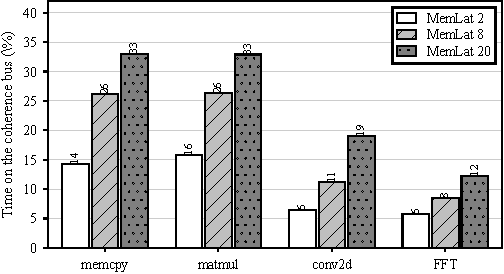
\includegraphics[width=\columnwidth]{fig_stall.pdf}
\caption{Time each core spends waiting for a snoopy-bus grant, as a percentage
of the cycles it had an access in the DCU. Table~\ref{tab:invuse} shows that
none of the traffic it is waiting for is necessary.}
\label{fig:stall}
\end{figure}

Between a twentieth and a third of a core's time goes to arbitrating for a
resource that grants one request per cycle across the whole cluster. The share
grows with memory latency, because each grant is held longer.

\subsection{It is not readers waiting on writers}

The obvious reading of Fig.~\ref{fig:stall} is contention between readers and
writers -- the single-writer screening doing its job. We instrumented the bus to
count it, and across all four kernels a read is \emph{never} withheld: not once.
Whatever the stall is, it is not the MRSW screening.

By elimination it is the invalidations, which are the only arbitrated traffic
left.

\subsection{None of the invalidations are necessary}

Each DCU therefore counts the broadcasts it receives and how many find a line to
clear. Table~\ref{tab:invuse} gives the result.

\begin{table}[t]
\caption{Invalidation broadcasts received across the cluster, and how many
invalidated a line. The last row is a control.}
\label{tab:invuse}
\centering
\begin{tabular}{@{}lrrr@{}}
\toprule
Workload & Broadcasts & Useful & \% \\
\midrule
matmul ($64^2$)      & 823{,}338 & 0 & 0.00 \\
conv2d ($64^2$)      & 139{,}182 & 0 & 0.00 \\
FFT ($N{=}256$)      &  61{,}683 & 0 & 0.00 \\
memcpy (16\,KiB)     &  24{,}618 & 0 & 0.00 \\
\midrule
sharing testbench    &       921 & 345 & 37.46 \\
\bottomrule
\end{tabular}
\end{table}

Over a million broadcasts, none of which invalidated anything. Each one paid a
cluster-wide arbitration and a four-way handshake to inform nobody of anything.

A result this uniform deserves suspicion of the instrument rather than of the
design, so the counter is controlled. Our coherence testbench shares
deliberately, with a producer/consumer ping-pong and a randomised four-core
stress over a small window; on that workload the same counter reports 345 useful
broadcasts of 921. The counter can see a useful invalidation. The zeroes are a
property of the workloads.

They are a property worth stating plainly: these kernels are data-parallel and
partition their data per core, so essentially every written line is private.
That is not a weakness of the benchmark selection, because these are the kernels
the original evaluation itself uses.

% =============================================================================
\section{An Exact Snoop Filter}
\label{sec:filter}
% =============================================================================

\subsection{Structure}

The bus needs to answer one question before granting an invalidation: is there
another cache that has to hear it? A mirror of the caches' tag and valid arrays
answers it, held in the bus and updated by the same two events that change the
caches themselves -- a refill installs a tag into a way, an invalidation clears
one. Each DCU exports those events on a small port driven from the same signals
that write its own arrays.

Exactness is therefore structural rather than argued. The mirror is written from
the same signals, on the same clock edge, under the same conditions as the state
it mirrors, so it cannot drift from it.

We rejected a hashed filter deliberately. A Bloom-style structure may only ever
over-approximate: claiming a line is held when it is not costs a redundant
broadcast and is safe, while the converse loses an invalidation and breaks
coherence. Insert-only hashed filters are safe but saturate, and matmul touches
far more lines than an affordable bitmap has bits; removing from one requires
knowing when a line leaves a cache, which is exactly the information a mirror
already has.

\subsection{Exact about the wrong property}
\label{sec:fill}

A mirror of the tag arrays is exact about which lines each cache \emph{holds},
and that turns out not to be the property the bus needs. A DCU between issuing
its memory read and refilling the victim way holds nothing for the line it is
fetching, so it does not appear in the mirror -- and it is precisely the cache
that must receive the invalidation, because receiving one in that window is what
cancels its refill. Suppress the broadcast and it installs a line that was
invalidated while in flight.

The property is residency \emph{or imminent residency}. Each DCU therefore
exports its refill window alongside its mirror updates, and the filter answers
over the union. The window opens when the cache issues the fetch and closes on
the cycle the refill lands, which is the same cycle the mirror learns the tag:
the two halves abut exactly, so the line is covered in every cycle by one or the
other.

This is not a defensive addition. Counting the granted invalidations for which
no other cache held the line but one was fetching it -- each one a broadcast a
committed-tag mirror would have wrongly suppressed -- our coherence testbench
reports 20 of 2{,}241 over ten randomised interleavings, and at least one in
every one of the ten. The window is narrow enough that the design passed 3{,}139
checks before the counter existed, which is how a race of this shape usually
survives a test suite.

\subsection{Why suppression is safe}

When the answer is that no other cache holds the line or is fetching it, a
broadcast could clear nothing anywhere, and not sending it is unobservable. That
is the whole argument, and it is short because the structure is exact. A
conservative filter would need an argument about the direction of its error;
this one needs only that it asks about the right state.

Everything else is untouched. Invalidations that \emph{are} needed are still
arbitrated, broadcast and acknowledged exactly as before; the single-writer
screening on reads is unchanged; and the write-through lock that stops a remote
read fetching a pre-write value is unchanged, because it protects against a
value in memory rather than against a cached copy.

\subsection{Implementation}

The mirror is one array per (core, way) pair, each with a single write port and
a single read port, addressed by set index -- eight arrays at the geometry
studied here. Tags are held outside any reset, since a tag is only compared when
its valid bit says it means something, which lets them map to distributed RAM.
Valid bits stay in flip-flops, where they can be reset and read eight at a time,
at 512 bits rather than 11{,}264. This is the same division the DCU makes
internally for the same reason.

That structure matters more than it might appear: a first implementation held
tags and valid bits together under an asynchronous reset and read them
combinationally, which Vivado mapped entirely to flip-flops -- 11{,}776 of them,
and 3{,}202 LUTs, against 512 and 408 for the structure above.

% =============================================================================
\section{Evaluation}
\label{sec:eval}
% =============================================================================

\subsection{Cycles}

\begin{figure*}[t]
\centering
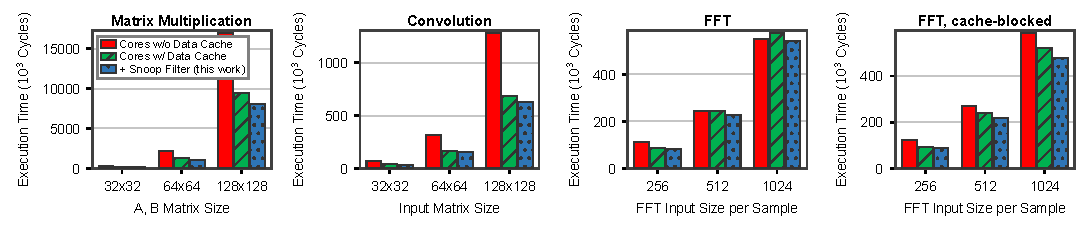
\includegraphics[width=\textwidth]{fig_exec.pdf}
\caption{Execution time of the three benchmark kernels against problem size,
without a data cache, with one, and with the snoop filter of this work. The
axes are those of the original's own execution-time figure, so the first two
bars of each cluster are directly comparable with it. Matrix multiplication and
convolution reproduce the reduction it reports; FFT does not, and the reason is
capacity rather than coherence -- see the text.}
\label{fig:exec}
\end{figure*}

Fig.~\ref{fig:exec} places the extension on the original's own axes: execution
time per kernel against problem size, uncached against cached, with our filter
added as a third bar the original has no counterpart to.

Two of the three reproduce it: matrix multiplication by 38.4 to 44.0\% and
convolution by 46 to 48\%, against the ${\approx}40\%$ the original reports for
both. Neither decays with problem size, and that is not luck. What must stay resident is not the data set but the \emph{reuse
footprint}, the bytes a core revisits before moving on -- one row of $B$ for
matrix multiplication, $4N$ bytes or 512\,B at $N{=}128$, and the three-row
sliding window for convolution, $12N$ bytes or 1536\,B. Both fit a 2\,KiB DCU
throughout, so the benefit does not move.

FFT is where that stops holding. The original reports a uniform
${\approx}23\%$; we match it at $N{=}256$, at 24.8\%, but the benefit falls to
0.4\% at 512 and turns negative at 1024, where the cache makes the kernel
\emph{slower} than having none. The footprint argument predicts exactly this:
FFT revisits $N$ complex points across its stages, $8N$ bytes, which is 2\,KiB
at $N{=}256$ and 8\,KiB at $N{=}1024$. Only the first fits.

That the cause is capacity and not conflict can be shown rather than asserted,
by moving one variable at a time. At $N{=}512$, doubling associativity at the
same 2\,KiB recovers 3.8\%; quadrupling capacity at the same associativity
recovers 24.5\%, and 16\,KiB recovers nothing beyond 8\,KiB. Saturation once the
footprint fits is the signature of a capacity limit, not a conflict one. Given a
DCU that holds the footprint, FFT then reproduces the original at every size --
24.8, 24.8 and 24.5\% at 8\,KiB. At the 2\,KiB its text states, it does not. We
read that as a configuration discrepancy rather than a contradiction: its result
implies a cache larger than the one specified, or a smaller working set, and the
published description does not let a reader tell which.

None of it weakens the filter, which is orthogonal: the filter removes coherence
traffic, not misses. It is worth roughly 50\% throughout on the first two
kernels, and at $N{=}1024$ it is what carries FFT back from $-4.3\%$ to parity.

%% The per-kernel speedup table was folded into the paragraph below. Three of
%% its four rows duplicated bars now in Fig. \ref{fig:exec}; what it uniquely
%% carried -- memcpy, and the oracle column -- is two sentences, and the page
%% limit was worth more than the fourth restatement of the same four numbers.

Against the unfiltered design the filter is worth $1.222\times$ on matrix
multiplication, $1.123\times$ on memcpy, $1.089\times$ on convolution and
$1.061\times$ on FFT: a geometric mean of $1.122\times$. The useful comparison
is not that mean but an oracle that suppresses every broadcast unconditionally,
which is sound to simulate only because Table~\ref{tab:invuse} says none are
needed, and which bounds what any filter could return.

%% fig_result removed to make room for fig_exec, which supersedes it: its panel
%% (a) plotted what the extension is worth against no cache, which fig_exec now
%% does for three kernels at three sizes rather than one size each. Its panel
%% (b), the snoop-stall reduction, survives as the numbers in the paragraph
%% below -- conv2d 20,848 to 109, memcpy 7,168 to 1 -- so no evidence is lost
%% with it. paper/fig_result.pdf is still generated by scripts/plot_date.py if
%% a venue with a looser page limit wants it back.

The filter reaches the oracle on every kernel, cycle for cycle. That is what an
exact structure should do on workloads with no sharing: it suppresses precisely
the broadcasts the oracle does, for a provable reason rather than an assumed
one.

The snoop-stall bucket confirms the mechanism rather than merely the outcome.
On conv2d it falls from 20{,}848 cycles to 109; on memcpy, from 7{,}168 to 1.
FFT is the exception and falls only from 6{,}521 to 2{,}955, because
load-reserved and store-conditional still pass the second arbiter whatever the
broadcasts do -- a residual cost no filter can remove.

\subsection{The extension stops being harmful}

The reproduction's most awkward finding was that on memcpy at low memory
latency, the cache extension is \emph{slower} than having no cache at all:
$0.975\times$ the non-coherent baseline. With the filter it runs at
$1.095\times$. The pathology is not intrinsic to attaching a coherent cache; it
is the cost of announcing private writes to a cluster that does not care.

\subsection{Coherence}

The four kernels never exercise the filter's must-broadcast path, so they cannot
establish that it is safe. Our coherence testbench does: it shares deliberately,
and roughly half of its invalidations are useful. With the filter enabled it
passes 3{,}112 checks, including a version-monotonicity invariant -- a core that
has observed version $k$ of a location may never afterwards observe a version
below $k$, which is exactly what a lost invalidation causes -- and a final
quiesce in which every core re-reads the whole window so that any line left
stale in any cache is caught against memory. The filter suppressed 282 of 921
broadcasts and delivered every one that mattered.

\subsection{FPGA cost}

Both configurations were implemented on a Zynq UltraScale+ XCZU7EV in a
non-project Vivado 2025.1 flow.

%% Per-module resource breakdown. Generated from
%%   python scripts/table1.py filtered
%% and transcribed here; regenerate that if the build changes.
%%
%% Single column, in the shape of the original's Table I: the module tree down
%% the left, then LUTs, FFs, BRAMs, DSPs, and Available / Utilisation rows
%% under the rule. The instance count is folded into the name and the LUTRAM
%% column is gone -- the one number from it that matters, the filter's 208
%% LUTRAM out of 408, is stated in the text where it is argued.
%%
%% Re-measured 2026-09-08 against the RTL that covers fills in flight, both
%% variants in one batch. No total row inside the tree on purpose: Vivado's
%% figure for the SoC is not the sum of the rows above it -- a LUT shared across
%% a hierarchy boundary counts against both children but once against the
%% parent -- so a total under the column would read as an arithmetic error. The
%% tool's own figures sit below the rule instead, where they are plainly a
%% separate statement.
\begin{table}[t]
\caption{Post-implementation resources, XCZU7EV at 60\,MHz, filtered build.
Sub-rows may sum slightly above their parent, because a LUT shared across a
hierarchy boundary is counted against both children but only once against the
parent. The figures below the rule are the tool's own, not column sums.}
\label{tab:fpga}
\centering
\footnotesize
\setlength{\tabcolsep}{3.5pt}
\begin{tabular}{@{}lrrrr@{}}
\toprule
Module & LUTs & FFs & BRAMs & DSPs \\
\midrule
\textbf{Processing element} ($\times$4)      & 17{,}833 & 9{,}948 & 32 & 20 \\
\quad RISC-V core, CV32E40P                  & 16{,}929 & 8{,}404 &  0 & 20 \\
\quad ITCM + Instr.-Bridge                   &      252 &      36 & 32 &  0 \\
\quad Data-Bridge                            &      319 &      32 &  0 &  0 \\
\quad AXI4 masters ($\times$3 per PE)        &      333 & 1{,}476 &  0 &  0 \\
\addlinespace[2pt]
\textbf{Cache extension}                     & \textbf{6{,}540} & \textbf{4{,}628} & 20 & 0 \\
\quad Data Cache Unit ($\times$4)            & 5{,}816 & 3{,}998 & 20 &  0 \\
\quad\quad controller + HCL                  & 2{,}860 & 2{,}846 &  0 &  0 \\
\quad\quad tag RAM                           & 1{,}677 &      96 &  4 &  0 \\
\quad\quad data RAM                          & 1{,}289 & 1{,}056 & 16 &  0 \\
\quad Snoopy bus                             &      728 &     630 &  0 &  0 \\
\quad\quad round-robin arbiter               &      251 &       2 &  0 &  0 \\
\quad\quad Invalidation Table                &       69 &     116 &  0 &  0 \\
\quad\quad \textbf{snoop filter (this work)} & \textbf{408} & \textbf{512} & 0 & 0 \\
\addlinespace[2pt]
\textbf{AXI4 crossbar}                       & 2{,}125 &     279 &  0 &  0 \\
\textbf{Shared data memory}, 256\,KiB        &      724 &     150 & 64 &  0 \\
\textbf{Shared instr.\ memory}, 32\,KiB      &      506 &      86 &  8 &  0 \\
\textbf{Control region}                      &      113 &     259 &  0 &  0 \\
\midrule
Whole device, as reported by the tool        & 27{,}845 & 15{,}670 & 124 & 20 \\
\addlinespace[1pt]
Available                                    & 230{,}400 & 460{,}800 & 312 & 1{,}728 \\
Utilisation (\%)                             &    12.09 &     3.40 & 39.74 & 1.16 \\
\bottomrule
\end{tabular}
\end{table}


Table~\ref{tab:fpga} gives the breakdown. The filter costs 1{,}064 LUTs and
516 flip-flops over the unfiltered design, under 4\% of it, and no block RAM or
DSP at all. Both configurations meet every constraint with no failing endpoints,
at $+1.199$~ns and $+1.265$~ns of slack respectively -- so at this operating
point the filter costs essentially no slack, 66~ps on a 16.667~ns period.

Both figures come from one source tree with one parameter changed, implemented
in the same batch, which is the only way a slack comparison on this design means
anything: an earlier pair of runs weeks apart put the same two configurations at
$+4.307$ and $+2.597$~ns, a 1.7~ns spread in the opposite direction, from
netlists differing by fourteen LUTs. Place-and-route outcomes move by more than
the effect being measured, so we quote slack only within a batch and never
across one.

Two things in the breakdown are worth drawing out. Half of the filter's 408
LUTs are distributed RAM holding the mirror, and its 512 flip-flops are exactly
the valid bits, four cores by 64 sets by two ways: the structure went in as
intended, with tags in memory and only the resettable state in registers. And
within the DCU the controller outweighs the storage, 2{,}802 LUTs against
1{,}677 for the tag array and 1{,}285 for the data array, because at 2\,KiB the
arrays are nearly free and the coherence logic is not.

\subsection{The frequency it costs}

It does cost frequency, and the paper would be misleading without saying so. At
a 75~MHz target the reference meets timing with $+1.327$~ns of slack and the
filtered design does not, at $-2.586$~ns. The critical path is 86\% routing and
runs from a DCU's registered request address across the die; the filter
lengthens it because the decision to broadcast is a cluster-spanning
combinational path, and it does so however the mirror is built. Making the
mirror smaller did not help: the flip-flop version above is four times the area
and closes \emph{better}, at $-0.423$~ns.

We therefore evaluate at 60~MHz, which both configurations meet comfortably, and
which is the frequency the original design itself runs at rather than one chosen
for convenience. At a fixed 60~MHz clock the filter's $1.122\times$ in cycles is
a $1.122\times$ in wall time. Clocked freely, the reference reaches a higher
frequency and the advantage narrows.

We deliberately do not report a maximum-frequency comparison from the 60~MHz
builds. Measured at a constraint that is already met, that figure records where
the tool stopped optimising rather than what the design can do: at 60~MHz it
favours the filtered design by 9.8~MHz, and at 75~MHz it favours the reference
by 20.5~MHz.

% =============================================================================
\section{What Did Not Work}
\label{sec:rejected}
% =============================================================================

Three mechanisms preceded this one. We report them because each was rejected by
a measurement that also sharpened the eventual design.

\textbf{A streaming mode} that would skip allocation and read at word
granularity for phases with no reuse. The non-coherent baseline already is such
a mode, and bounds it: on memcpy it beats the cache at a memory latency of two
by 2.5\% and loses by better than two to one at eight and twenty, because a line
fill amortises one memory latency across four words.

\textbf{A hit-speculative bypass}, in which a read presumes it will hit and
takes no bus transaction, and only a miss arbitrates. It was both useless and
incorrect. Useless because plain reads were never arbitrated in the first place,
so there was no cost to remove -- it measured slower. Incorrect because the
screening it removed is not about allocation but is the single-writer half of
MRSW: a read that hits a resident line while a remote invalidation for that line
is outstanding returns stale data. It passed all eleven functional checks of the
benchmark harness, which is the point worth reporting: the race window is narrow
and a green test said nothing about it.

\textbf{Two structural fixes to the mirror}, described in
Section~\ref{sec:eval}: neither the register count nor the storage type was the
cause of the frequency loss.

\textbf{Directed invalidation}, the obvious next step, which does not pay. The
mirror knows not merely \emph{whether} another cache holds the line but
\emph{which} ones do, so the bus can invalidate exactly those and hold the grant
on only those: an exact multicast with a partial barrier. Only an exact filter
may do this, since under multicast a missing sharer bit loses an invalidation
rather than costing a redundant broadcast. Measured on a halo-exchange stencil
whose band boundaries give a sharer set of exactly one of three, it behaves
perfectly -- 168 invalidations delivered, all 168 useful, against suppression's
504, with the residual stall down elevenfold -- and is worth 0.1 to 0.3\% at
every memory latency tried. Exact suppression has already removed the traffic
that caused the serialisation, and the remainder is irreducible: somebody does
have to be told, and the writer does have to wait. Once the filter is exact, the
residue is not worth steering.

% =============================================================================
\section{Threats to Validity}
% =============================================================================

The central measurement is that none of the invalidation traffic is useful, and
that is a property of workloads as much as of the design. Data-parallel kernels
that partition per core have almost nothing to share. We claim only what we
measured: on the kernels the original evaluation itself uses, this design's
coherence traffic is entirely avoidable. The halo-exchange stencil of
Section~\ref{sec:rejected} is the case with genuine sharing, and the filter is
still worth $1.11\times$ there at a memory latency of twenty, because the
interior of each band is private even when its boundary is not. Our coherence
testbench, at roughly half its invalidations useful, is the extreme in the other
direction.

The evaluation is in cycles from RTL simulation and in post-place-and-route
resource and timing figures; no bitstream has been run on hardware. The original
targets a Virtex UltraScale+ XCVU9P and this work an XCZU7EV, so absolute
figures are directional rather than a like-for-like comparison.

Power is not reported: Vivado's vectorless estimate models this design as idle,
because it cannot evaluate the cores' clock-gate enables.

% =============================================================================
\section{Conclusion}
% =============================================================================

A seamless coherent cache extension for soft RISC-V multicores spends between 6
and 33\% of each core's time on a coherence protocol that, on its own benchmark
kernels, accomplishes nothing: over a million invalidation broadcasts, none of
which invalidate anything. An exact mirror of the caches' tag arrays lets the
bus suppress those broadcasts for 1{,}064 LUTs and 516 flip-flops, preserving
coherence structurally rather than by argument, and is worth a geometric mean
$1.122\times$ at a fixed 60~MHz clock. It also removes the case in which the
extension was slower than having no cache at all. The mechanism costs
frequency, and we report where that matters.

\ifanon
\else
The design, the measurements and the scripts that regenerate every table are
available at \url{https://github.com/Krishna-Gorai/riscv-cache-extension}.
\fi

\begin{thebibliography}{1}
\bibitem{kamaleldin2024}
A.~Kamaleldin, M.~Nickel, S.~Wu and D.~G\"ohringer,
``Seamless Cache Extension for FPGA-based Multi-Core RISC-V SoC,''
in \emph{Proc. IEEE 37th Int. System-on-Chip Conf. (SOCC)}, 2024.

\bibitem{jetty}
A.~Moshovos, G.~Memik, B.~Falsafi and A.~Choudhary,
``JETTY: Filtering Snoops for Reduced Energy Consumption in SMP Servers,''
in \emph{Proc. 7th Int. Symp. High-Performance Computer Architecture (HPCA)},
2001.

\bibitem{cgct}
J.~F.~Cantin, M.~H.~Lipasti and J.~E.~Smith,
``Improving Multiprocessor Performance with Coarse-Grain Coherence Tracking,''
in \emph{Proc. 32nd Int. Symp. Computer Architecture (ISCA)}, 2005, pp.
246--257.

\bibitem{regionscout}
A.~Moshovos,
``RegionScout: Exploiting Coarse Grain Sharing in Snoop-Based Coherence,''
in \emph{Proc. 32nd Int. Symp. Computer Architecture (ISCA)}, 2005, pp.
234--245.

\bibitem{tilelink}
W.~Terpstra,
``TileLink: A Free and Open-Source, High-Performance Scalable Cache-Coherent
Fabric Designed for RISC-V,'' in \emph{RISC-V Workshop}, 2017.

\bibitem{openpiton}
J.~Balkind \emph{et al.},
``OpenPiton+Ariane: The First Open-Source, SMP Linux-booting RISC-V System
Scaling from One to Many Cores,'' in \emph{Workshop on Computer Architecture
Research with RISC-V (CARRV)}, 2019.

\bibitem{cifer}
A.~Li \emph{et al.},
``CIFER: A Cache-Coherent 12nm 16mm$^2$ SoC with Four 64-Bit RISC-V Application
Cores, 18 32-Bit RISC-V Compute Cores, and a 1541 LUT6/mm$^2$ Synthesizable
eFPGA,'' in \emph{IEEE Int. Solid-State Circuits Conf. (ISSCC)}, 2023.
\end{thebibliography}

\end{document}
"
%%
%%  Defaults to anonymous. DATE's blind-review policy for the research track
%%  must be confirmed before submission -- the repository URL de-anonymises the
%%  work instantly, so it is behind the same toggle as the author block.
%% =============================================================================
\documentclass[conference]{IEEEtran}
\IEEEoverridecommandlockouts

\usepackage{cite}
\usepackage{amsmath,amssymb}
\usepackage{graphicx}
\usepackage{booktabs}
\usepackage{url}
\usepackage[hidelinks]{hyperref}

\ifdefined\CAMERAREADY \newif\ifanon \anonfalse \else \newif\ifanon \anontrue \fi

\begin{document}

\title{An Exact Snoop Filter for Seamless Cache Coherence in
FPGA-Based Multi-Core RISC-V}

\ifanon
  \author{\IEEEauthorblockN{Anonymous submission}}
\else
  \author{\IEEEauthorblockN{Krishna Gorai}
  \IEEEauthorblockA{Indian Institute of Technology Mandi\\
  Mandi, Himachal Pradesh, India}
  \and
  \IEEEauthorblockN{Bikram Paul}
  \IEEEauthorblockA{Indian Institute of Technology Mandi\\
  Mandi, Himachal Pradesh, India}}
\fi

\maketitle

\begin{abstract}
Attaching a private, snoop-coherent L1 data cache to an unmodified RISC-V core
is an attractive way to build FPGA multi-core systems, and a recently proposed
design does so with coherence handled entirely in hardware. We reproduce that
design in open-source RTL and measure where its time actually goes. Across four
benchmark kernels the cluster issues 1{,}048{,}821 invalidation broadcasts and
not one of them invalidates a line in another cache. Every kernel partitions its
data per processing element, so every written line is private, yet each write
still pays a cluster-wide arbitration and a handshake that waits on every other
cache. That accounts for between 6 and 33\% of a core's execution time, and on a
streaming kernel it makes the cache extension slower than having no cache at
all. We add a snoop filter that keeps an exact mirror of the caches' tag arrays
and suppresses a broadcast when no other cache holds the line or is fetching it
-- a distinction that is not cosmetic, since a mirror of committed tags alone
loses invalidations. It costs 1{,}064
LUTs and 516 flip-flops, preserves coherence under a version-monotonicity
checker, and is worth a geometric mean $1.12\times$, up to $1.22\times$ on
matrix multiplication. It also converts the streaming kernel from $0.98\times$
to $1.10\times$ against an uncached baseline. We report the frequency it costs,
and evaluate at the original design's own 60~MHz operating point.
\end{abstract}

\begin{IEEEkeywords}
RISC-V, cache coherence, snoop filter, FPGA, multi-core
\end{IEEEkeywords}

% =============================================================================
\section{Introduction}
% =============================================================================

A soft multi-core system on an FPGA gains a great deal from being able to attach
a data cache to an existing, verified RISC-V core without modifying it. The core
stays an unmodified IP block, coherence is handled in hardware, and software
needs no knowledge of either. Kamaleldin \emph{et al.}~\cite{kamaleldin2024}
propose exactly this: a private write-through L1 data cache unit (DCU) attached
through the core's ordinary memory interface, with a snooping invalidation bus
maintaining coherence across the cluster.

We built that design from scratch in open-source SystemVerilog in order to
measure it, and the measurement is the origin of this paper. The DCU exports
per-access cycle accounting, and it says that between 6 and 33\% of a core's
time is spent waiting on the coherence bus. That is a large number for a
mechanism that, on these workloads, turns out to accomplish nothing at all:
across four kernels the cluster sends 1{,}048{,}821 invalidation broadcasts and
none of them invalidates a line anywhere.

The reason is structural rather than accidental. The kernels are data-parallel
and partition their arrays per processing element, so almost every written line
is private to the core writing it. The bus has no way to know that, so every
write is announced to every cache, and the announcement is serialised: at most
one invalidation is granted per cycle, and the grant is withheld until every
other cache is ready to accept the broadcast.

Our contributions are:

\begin{itemize}
  \item A measurement of how much of this design's coherence traffic is
        necessary. On its own benchmark kernels, none of it is, and we quantify
        what that costs (Section~\ref{sec:measure}).
  \item An exact snoop filter: a structural mirror of the caches' tag arrays
        that lets the bus suppress a broadcast no cache needs. Exactness has to
        be over the right property -- a mirror of committed tags alone is
        unsound, because a cache with a refill in flight holds nothing yet and
        must still be told -- and we measure how often that distinction decides
        a coherence violation (Section~\ref{sec:filter}).
  \item An evaluation in cycles, in coherence correctness, and in
        place-and-routed FPGA cost, including the frequency the mechanism costs
        and the operating point at which it pays (Section~\ref{sec:eval}).
  \item Three mechanisms we designed, measured and rejected before this one,
        including one that was incorrect while passing every functional test it
        had (Section~\ref{sec:rejected}).
\end{itemize}

% =============================================================================
\section{Related Work}
% =============================================================================

Filtering snoops is not a new idea, and the value here is not the concept but
where the filter sits, what it is exact about, and what it is measured against.

JETTY~\cite{jetty} places a small cache-like structure between the bus and each
processor's L2, filtering snoops that would miss locally so that the energy of a
tag lookup is not spent. Its target is energy, its position is the receiving
side, and it is approximate: a small JETTY filters most useless snoops, not all.
Coarse-grain coherence tracking~\cite{cgct} and RegionScout~\cite{regionscout}
raise the granularity instead, tracking sharing over regions of hundreds or
thousands of bytes so that a region known to be unshared needs no broadcast at
all, trading precision for a much smaller structure.

Our setting inverts the cost that matters. On a snooping bus in a soft
multi-core, the expense of an unnecessary invalidation is not the energy of the
remote tag lookups but the \emph{serialisation}: one grant per cycle across the
cluster, held until every other cache is ready to accept the broadcast. The
filter therefore belongs at the source, deciding whether to arbitrate at all,
rather than at each receiver deciding whether to look. And because the design is
small -- four caches of 128 lines each -- an exact mirror is affordable, at
1{,}064 LUTs (Section~\ref{sec:eval}), which removes the need to trade precision
for size and reduces the correctness argument to a sentence. A region-based
scheme would be the right choice at a scale where an exact mirror is not
affordable; at this one it is not necessary.

The RISC-V ecosystem offers coherent fabrics at a range of scales:
TileLink~\cite{tilelink} as a coherent interconnect standard,
OpenPiton~\cite{openpiton} scaling directory coherence to many cores, and
CIFER~\cite{cifer} integrating coherent clusters in silicon. These are complete
memory systems, and adopting one means adopting its interconnect. The design
studied here occupies a deliberately different point: an extension attached to
an unmodified core through its existing memory port, which is what makes it
attractive on an FPGA and also what confines coherence to a single shared bus.
Our contribution is to that design point, not to coherent fabrics generally.

Finally, the measurement itself has a precedent worth acknowledging. JETTY's
premise is the observation that many snoops find no copy elsewhere. On the
benchmark kernels of the design studied here, \emph{no} invalidation finds a
copy elsewhere -- Section~\ref{sec:measure} establishes that, and it is the
result the rest of this paper follows from. The difference between "many" and
"all" is a property of data-parallel workloads on a private-cache cluster, and
it is what makes an exact filter worth its area here.

% =============================================================================
\section{The Design Under Study}
% =============================================================================

\begin{figure*}[t]
\centering
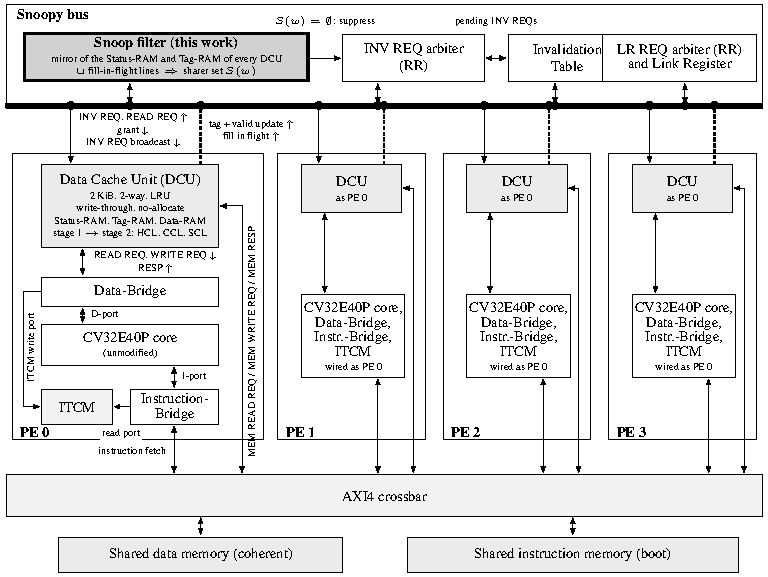
\includegraphics[width=\textwidth]{fig_arch.pdf}
\caption{The system, and what this work adds to it. Four unmodified cores sit
over their private data cache units, which reach shared memory through an AXI4
crossbar and maintain coherence through a single snoopy bus. The snoop filter
holds a mirror of every cache's tag and valid arrays, kept current by one update
port per DCU, and answers the invalidation arbiter's one question: is there
anybody to tell?}
\label{fig:arch}
\end{figure*}

The DCU is a private, write-through, no-allocate L1 data cache sitting between
an in-order RISC-V core and the memory system. Because writes go through to
memory, shared memory always holds the current value and no dirty-line writeback
or ownership state is needed. Coherence is maintained by an invalidation bus:
a core write reaches the bus as an invalidation request, and on grant the
address is broadcast to every other DCU, which drops any matching line.

Two properties of that bus matter here. Plain read requests are not arbitrated
against each other -- multiple readers proceed in the same cycle, which is the
multiple-readers half of the MRSW invariant -- but a read is withheld while
another core has an invalidation outstanding for the same line, which is the
single-writer half. Invalidations \emph{are} arbitrated: at most one is granted
per cycle across the cluster, and the grant is held back until every other DCU
can accept the broadcast, so that no invalidation is ever lost.

Fig.~\ref{fig:arch} shows the system and where the filter sits in it.
Our reproduction targets the stated configuration: four processing elements,
each an unmodified CV32E40P with a private 2\,KiB two-way DCU of 16-byte lines,
meeting shared memories through an AXI4 crossbar. A non-coherent baseline is
built from the same sources with one parameter changed, so any comparison
between them is attributable to the cache sub-system alone.

% =============================================================================
\section{Where the Time Goes}
\label{sec:measure}
% =============================================================================

\subsection{The coherence bus is a large fraction of runtime}

The DCU separates a core access into the places it can wait. One of those is
stage~1 waiting for a snoopy-bus grant. Fig.~\ref{fig:stall} gives that bucket
as a fraction of the cycles a core spent with an access in the DCU at all,
for each kernel at three memory latencies.

\begin{figure}[t]
\centering
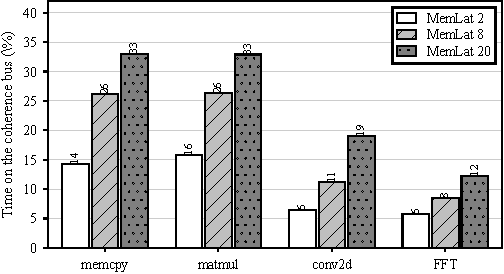
\includegraphics[width=\columnwidth]{fig_stall.pdf}
\caption{Time each core spends waiting for a snoopy-bus grant, as a percentage
of the cycles it had an access in the DCU. Table~\ref{tab:invuse} shows that
none of the traffic it is waiting for is necessary.}
\label{fig:stall}
\end{figure}

Between a twentieth and a third of a core's time goes to arbitrating for a
resource that grants one request per cycle across the whole cluster. The share
grows with memory latency, because each grant is held longer.

\subsection{It is not readers waiting on writers}

The obvious reading of Fig.~\ref{fig:stall} is contention between readers and
writers -- the single-writer screening doing its job. We instrumented the bus to
count it, and across all four kernels a read is \emph{never} withheld: not once.
Whatever the stall is, it is not the MRSW screening.

By elimination it is the invalidations, which are the only arbitrated traffic
left.

\subsection{None of the invalidations are necessary}

Each DCU therefore counts the broadcasts it receives and how many find a line to
clear. Table~\ref{tab:invuse} gives the result.

\begin{table}[t]
\caption{Invalidation broadcasts received across the cluster, and how many
invalidated a line. The last row is a control.}
\label{tab:invuse}
\centering
\begin{tabular}{@{}lrrr@{}}
\toprule
Workload & Broadcasts & Useful & \% \\
\midrule
matmul ($64^2$)      & 823{,}338 & 0 & 0.00 \\
conv2d ($64^2$)      & 139{,}182 & 0 & 0.00 \\
FFT ($N{=}256$)      &  61{,}683 & 0 & 0.00 \\
memcpy (16\,KiB)     &  24{,}618 & 0 & 0.00 \\
\midrule
sharing testbench    &       921 & 345 & 37.46 \\
\bottomrule
\end{tabular}
\end{table}

Over a million broadcasts, none of which invalidated anything. Each one paid a
cluster-wide arbitration and a four-way handshake to inform nobody of anything.

A result this uniform deserves suspicion of the instrument rather than of the
design, so the counter is controlled. Our coherence testbench shares
deliberately, with a producer/consumer ping-pong and a randomised four-core
stress over a small window; on that workload the same counter reports 345 useful
broadcasts of 921. The counter can see a useful invalidation. The zeroes are a
property of the workloads.

They are a property worth stating plainly: these kernels are data-parallel and
partition their data per core, so essentially every written line is private.
That is not a weakness of the benchmark selection, because these are the kernels
the original evaluation itself uses.

% =============================================================================
\section{An Exact Snoop Filter}
\label{sec:filter}
% =============================================================================

\subsection{Structure}

The bus needs to answer one question before granting an invalidation: is there
another cache that has to hear it? A mirror of the caches' tag and valid arrays
answers it, held in the bus and updated by the same two events that change the
caches themselves -- a refill installs a tag into a way, an invalidation clears
one. Each DCU exports those events on a small port driven from the same signals
that write its own arrays.

Exactness is therefore structural rather than argued. The mirror is written from
the same signals, on the same clock edge, under the same conditions as the state
it mirrors, so it cannot drift from it.

We rejected a hashed filter deliberately. A Bloom-style structure may only ever
over-approximate: claiming a line is held when it is not costs a redundant
broadcast and is safe, while the converse loses an invalidation and breaks
coherence. Insert-only hashed filters are safe but saturate, and matmul touches
far more lines than an affordable bitmap has bits; removing from one requires
knowing when a line leaves a cache, which is exactly the information a mirror
already has.

\subsection{Exact about the wrong property}
\label{sec:fill}

A mirror of the tag arrays is exact about which lines each cache \emph{holds},
and that turns out not to be the property the bus needs. A DCU between issuing
its memory read and refilling the victim way holds nothing for the line it is
fetching, so it does not appear in the mirror -- and it is precisely the cache
that must receive the invalidation, because receiving one in that window is what
cancels its refill. Suppress the broadcast and it installs a line that was
invalidated while in flight.

The property is residency \emph{or imminent residency}. Each DCU therefore
exports its refill window alongside its mirror updates, and the filter answers
over the union. The window opens when the cache issues the fetch and closes on
the cycle the refill lands, which is the same cycle the mirror learns the tag:
the two halves abut exactly, so the line is covered in every cycle by one or the
other.

This is not a defensive addition. Counting the granted invalidations for which
no other cache held the line but one was fetching it -- each one a broadcast a
committed-tag mirror would have wrongly suppressed -- our coherence testbench
reports 20 of 2{,}241 over ten randomised interleavings, and at least one in
every one of the ten. The window is narrow enough that the design passed 3{,}139
checks before the counter existed, which is how a race of this shape usually
survives a test suite.

\subsection{Why suppression is safe}

When the answer is that no other cache holds the line or is fetching it, a
broadcast could clear nothing anywhere, and not sending it is unobservable. That
is the whole argument, and it is short because the structure is exact. A
conservative filter would need an argument about the direction of its error;
this one needs only that it asks about the right state.

Everything else is untouched. Invalidations that \emph{are} needed are still
arbitrated, broadcast and acknowledged exactly as before; the single-writer
screening on reads is unchanged; and the write-through lock that stops a remote
read fetching a pre-write value is unchanged, because it protects against a
value in memory rather than against a cached copy.

\subsection{Implementation}

The mirror is one array per (core, way) pair, each with a single write port and
a single read port, addressed by set index -- eight arrays at the geometry
studied here. Tags are held outside any reset, since a tag is only compared when
its valid bit says it means something, which lets them map to distributed RAM.
Valid bits stay in flip-flops, where they can be reset and read eight at a time,
at 512 bits rather than 11{,}264. This is the same division the DCU makes
internally for the same reason.

That structure matters more than it might appear: a first implementation held
tags and valid bits together under an asynchronous reset and read them
combinationally, which Vivado mapped entirely to flip-flops -- 11{,}776 of them,
and 3{,}202 LUTs, against 512 and 408 for the structure above.

% =============================================================================
\section{Evaluation}
\label{sec:eval}
% =============================================================================

\subsection{Cycles}

\begin{figure*}[t]
\centering
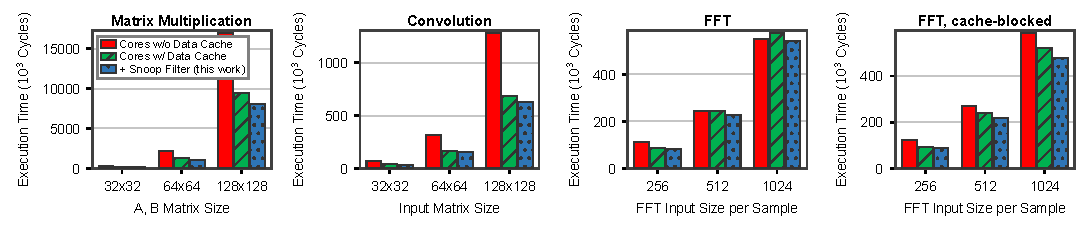
\includegraphics[width=\textwidth]{fig_exec.pdf}
\caption{Execution time of the three benchmark kernels against problem size,
without a data cache, with one, and with the snoop filter of this work. The
axes are those of the original's own execution-time figure, so the first two
bars of each cluster are directly comparable with it. Matrix multiplication and
convolution reproduce the reduction it reports; FFT does not, and the reason is
capacity rather than coherence -- see the text.}
\label{fig:exec}
\end{figure*}

Fig.~\ref{fig:exec} places the extension on the original's own axes: execution
time per kernel against problem size, uncached against cached, with our filter
added as a third bar the original has no counterpart to.

Two of the three reproduce it: matrix multiplication by 38.4 to 44.0\% and
convolution by 46 to 48\%, against the ${\approx}40\%$ the original reports for
both. Neither decays with problem size, and that is not luck. What must stay resident is not the data set but the \emph{reuse
footprint}, the bytes a core revisits before moving on -- one row of $B$ for
matrix multiplication, $4N$ bytes or 512\,B at $N{=}128$, and the three-row
sliding window for convolution, $12N$ bytes or 1536\,B. Both fit a 2\,KiB DCU
throughout, so the benefit does not move.

FFT is where that stops holding. The original reports a uniform
${\approx}23\%$; we match it at $N{=}256$, at 24.8\%, but the benefit falls to
0.4\% at 512 and turns negative at 1024, where the cache makes the kernel
\emph{slower} than having none. The footprint argument predicts exactly this:
FFT revisits $N$ complex points across its stages, $8N$ bytes, which is 2\,KiB
at $N{=}256$ and 8\,KiB at $N{=}1024$. Only the first fits.

That the cause is capacity and not conflict can be shown rather than asserted,
by moving one variable at a time. At $N{=}512$, doubling associativity at the
same 2\,KiB recovers 3.8\%; quadrupling capacity at the same associativity
recovers 24.5\%, and 16\,KiB recovers nothing beyond 8\,KiB. Saturation once the
footprint fits is the signature of a capacity limit, not a conflict one. Given a
DCU that holds the footprint, FFT then reproduces the original at every size --
24.8, 24.8 and 24.5\% at 8\,KiB. At the 2\,KiB its text states, it does not. We
read that as a configuration discrepancy rather than a contradiction: its result
implies a cache larger than the one specified, or a smaller working set, and the
published description does not let a reader tell which.

None of it weakens the filter, which is orthogonal: the filter removes coherence
traffic, not misses. It is worth roughly 50\% throughout on the first two
kernels, and at $N{=}1024$ it is what carries FFT back from $-4.3\%$ to parity.

%% The per-kernel speedup table was folded into the paragraph below. Three of
%% its four rows duplicated bars now in Fig. \ref{fig:exec}; what it uniquely
%% carried -- memcpy, and the oracle column -- is two sentences, and the page
%% limit was worth more than the fourth restatement of the same four numbers.

Against the unfiltered design the filter is worth $1.222\times$ on matrix
multiplication, $1.123\times$ on memcpy, $1.089\times$ on convolution and
$1.061\times$ on FFT: a geometric mean of $1.122\times$. The useful comparison
is not that mean but an oracle that suppresses every broadcast unconditionally,
which is sound to simulate only because Table~\ref{tab:invuse} says none are
needed, and which bounds what any filter could return.

%% fig_result removed to make room for fig_exec, which supersedes it: its panel
%% (a) plotted what the extension is worth against no cache, which fig_exec now
%% does for three kernels at three sizes rather than one size each. Its panel
%% (b), the snoop-stall reduction, survives as the numbers in the paragraph
%% below -- conv2d 20,848 to 109, memcpy 7,168 to 1 -- so no evidence is lost
%% with it. paper/fig_result.pdf is still generated by scripts/plot_date.py if
%% a venue with a looser page limit wants it back.

The filter reaches the oracle on every kernel, cycle for cycle. That is what an
exact structure should do on workloads with no sharing: it suppresses precisely
the broadcasts the oracle does, for a provable reason rather than an assumed
one.

The snoop-stall bucket confirms the mechanism rather than merely the outcome.
On conv2d it falls from 20{,}848 cycles to 109; on memcpy, from 7{,}168 to 1.
FFT is the exception and falls only from 6{,}521 to 2{,}955, because
load-reserved and store-conditional still pass the second arbiter whatever the
broadcasts do -- a residual cost no filter can remove.

\subsection{The extension stops being harmful}

The reproduction's most awkward finding was that on memcpy at low memory
latency, the cache extension is \emph{slower} than having no cache at all:
$0.975\times$ the non-coherent baseline. With the filter it runs at
$1.095\times$. The pathology is not intrinsic to attaching a coherent cache; it
is the cost of announcing private writes to a cluster that does not care.

\subsection{Coherence}

The four kernels never exercise the filter's must-broadcast path, so they cannot
establish that it is safe. Our coherence testbench does: it shares deliberately,
and roughly half of its invalidations are useful. With the filter enabled it
passes 3{,}112 checks, including a version-monotonicity invariant -- a core that
has observed version $k$ of a location may never afterwards observe a version
below $k$, which is exactly what a lost invalidation causes -- and a final
quiesce in which every core re-reads the whole window so that any line left
stale in any cache is caught against memory. The filter suppressed 282 of 921
broadcasts and delivered every one that mattered.

\subsection{FPGA cost}

Both configurations were implemented on a Zynq UltraScale+ XCZU7EV in a
non-project Vivado 2025.1 flow.

%% Per-module resource breakdown. Generated from
%%   python scripts/table1.py filtered
%% and transcribed here; regenerate that if the build changes.
%%
%% Single column, in the shape of the original's Table I: the module tree down
%% the left, then LUTs, FFs, BRAMs, DSPs, and Available / Utilisation rows
%% under the rule. The instance count is folded into the name and the LUTRAM
%% column is gone -- the one number from it that matters, the filter's 208
%% LUTRAM out of 408, is stated in the text where it is argued.
%%
%% Re-measured 2026-09-08 against the RTL that covers fills in flight, both
%% variants in one batch. No total row inside the tree on purpose: Vivado's
%% figure for the SoC is not the sum of the rows above it -- a LUT shared across
%% a hierarchy boundary counts against both children but once against the
%% parent -- so a total under the column would read as an arithmetic error. The
%% tool's own figures sit below the rule instead, where they are plainly a
%% separate statement.
\begin{table}[t]
\caption{Post-implementation resources, XCZU7EV at 60\,MHz, filtered build.
Sub-rows may sum slightly above their parent, because a LUT shared across a
hierarchy boundary is counted against both children but only once against the
parent. The figures below the rule are the tool's own, not column sums.}
\label{tab:fpga}
\centering
\footnotesize
\setlength{\tabcolsep}{3.5pt}
\begin{tabular}{@{}lrrrr@{}}
\toprule
Module & LUTs & FFs & BRAMs & DSPs \\
\midrule
\textbf{Processing element} ($\times$4)      & 17{,}833 & 9{,}948 & 32 & 20 \\
\quad RISC-V core, CV32E40P                  & 16{,}929 & 8{,}404 &  0 & 20 \\
\quad ITCM + Instr.-Bridge                   &      252 &      36 & 32 &  0 \\
\quad Data-Bridge                            &      319 &      32 &  0 &  0 \\
\quad AXI4 masters ($\times$3 per PE)        &      333 & 1{,}476 &  0 &  0 \\
\addlinespace[2pt]
\textbf{Cache extension}                     & \textbf{6{,}540} & \textbf{4{,}628} & 20 & 0 \\
\quad Data Cache Unit ($\times$4)            & 5{,}816 & 3{,}998 & 20 &  0 \\
\quad\quad controller + HCL                  & 2{,}860 & 2{,}846 &  0 &  0 \\
\quad\quad tag RAM                           & 1{,}677 &      96 &  4 &  0 \\
\quad\quad data RAM                          & 1{,}289 & 1{,}056 & 16 &  0 \\
\quad Snoopy bus                             &      728 &     630 &  0 &  0 \\
\quad\quad round-robin arbiter               &      251 &       2 &  0 &  0 \\
\quad\quad Invalidation Table                &       69 &     116 &  0 &  0 \\
\quad\quad \textbf{snoop filter (this work)} & \textbf{408} & \textbf{512} & 0 & 0 \\
\addlinespace[2pt]
\textbf{AXI4 crossbar}                       & 2{,}125 &     279 &  0 &  0 \\
\textbf{Shared data memory}, 256\,KiB        &      724 &     150 & 64 &  0 \\
\textbf{Shared instr.\ memory}, 32\,KiB      &      506 &      86 &  8 &  0 \\
\textbf{Control region}                      &      113 &     259 &  0 &  0 \\
\midrule
Whole device, as reported by the tool        & 27{,}845 & 15{,}670 & 124 & 20 \\
\addlinespace[1pt]
Available                                    & 230{,}400 & 460{,}800 & 312 & 1{,}728 \\
Utilisation (\%)                             &    12.09 &     3.40 & 39.74 & 1.16 \\
\bottomrule
\end{tabular}
\end{table}


Table~\ref{tab:fpga} gives the breakdown. The filter costs 1{,}064 LUTs and
516 flip-flops over the unfiltered design, under 4\% of it, and no block RAM or
DSP at all. Both configurations meet every constraint with no failing endpoints,
at $+1.199$~ns and $+1.265$~ns of slack respectively -- so at this operating
point the filter costs essentially no slack, 66~ps on a 16.667~ns period.

Both figures come from one source tree with one parameter changed, implemented
in the same batch, which is the only way a slack comparison on this design means
anything: an earlier pair of runs weeks apart put the same two configurations at
$+4.307$ and $+2.597$~ns, a 1.7~ns spread in the opposite direction, from
netlists differing by fourteen LUTs. Place-and-route outcomes move by more than
the effect being measured, so we quote slack only within a batch and never
across one.

Two things in the breakdown are worth drawing out. Half of the filter's 408
LUTs are distributed RAM holding the mirror, and its 512 flip-flops are exactly
the valid bits, four cores by 64 sets by two ways: the structure went in as
intended, with tags in memory and only the resettable state in registers. And
within the DCU the controller outweighs the storage, 2{,}802 LUTs against
1{,}677 for the tag array and 1{,}285 for the data array, because at 2\,KiB the
arrays are nearly free and the coherence logic is not.

\subsection{The frequency it costs}

It does cost frequency, and the paper would be misleading without saying so. At
a 75~MHz target the reference meets timing with $+1.327$~ns of slack and the
filtered design does not, at $-2.586$~ns. The critical path is 86\% routing and
runs from a DCU's registered request address across the die; the filter
lengthens it because the decision to broadcast is a cluster-spanning
combinational path, and it does so however the mirror is built. Making the
mirror smaller did not help: the flip-flop version above is four times the area
and closes \emph{better}, at $-0.423$~ns.

We therefore evaluate at 60~MHz, which both configurations meet comfortably, and
which is the frequency the original design itself runs at rather than one chosen
for convenience. At a fixed 60~MHz clock the filter's $1.122\times$ in cycles is
a $1.122\times$ in wall time. Clocked freely, the reference reaches a higher
frequency and the advantage narrows.

We deliberately do not report a maximum-frequency comparison from the 60~MHz
builds. Measured at a constraint that is already met, that figure records where
the tool stopped optimising rather than what the design can do: at 60~MHz it
favours the filtered design by 9.8~MHz, and at 75~MHz it favours the reference
by 20.5~MHz.

% =============================================================================
\section{What Did Not Work}
\label{sec:rejected}
% =============================================================================

Three mechanisms preceded this one. We report them because each was rejected by
a measurement that also sharpened the eventual design.

\textbf{A streaming mode} that would skip allocation and read at word
granularity for phases with no reuse. The non-coherent baseline already is such
a mode, and bounds it: on memcpy it beats the cache at a memory latency of two
by 2.5\% and loses by better than two to one at eight and twenty, because a line
fill amortises one memory latency across four words.

\textbf{A hit-speculative bypass}, in which a read presumes it will hit and
takes no bus transaction, and only a miss arbitrates. It was both useless and
incorrect. Useless because plain reads were never arbitrated in the first place,
so there was no cost to remove -- it measured slower. Incorrect because the
screening it removed is not about allocation but is the single-writer half of
MRSW: a read that hits a resident line while a remote invalidation for that line
is outstanding returns stale data. It passed all eleven functional checks of the
benchmark harness, which is the point worth reporting: the race window is narrow
and a green test said nothing about it.

\textbf{Two structural fixes to the mirror}, described in
Section~\ref{sec:eval}: neither the register count nor the storage type was the
cause of the frequency loss.

\textbf{Directed invalidation}, the obvious next step, which does not pay. The
mirror knows not merely \emph{whether} another cache holds the line but
\emph{which} ones do, so the bus can invalidate exactly those and hold the grant
on only those: an exact multicast with a partial barrier. Only an exact filter
may do this, since under multicast a missing sharer bit loses an invalidation
rather than costing a redundant broadcast. Measured on a halo-exchange stencil
whose band boundaries give a sharer set of exactly one of three, it behaves
perfectly -- 168 invalidations delivered, all 168 useful, against suppression's
504, with the residual stall down elevenfold -- and is worth 0.1 to 0.3\% at
every memory latency tried. Exact suppression has already removed the traffic
that caused the serialisation, and the remainder is irreducible: somebody does
have to be told, and the writer does have to wait. Once the filter is exact, the
residue is not worth steering.

% =============================================================================
\section{Threats to Validity}
% =============================================================================

The central measurement is that none of the invalidation traffic is useful, and
that is a property of workloads as much as of the design. Data-parallel kernels
that partition per core have almost nothing to share. We claim only what we
measured: on the kernels the original evaluation itself uses, this design's
coherence traffic is entirely avoidable. The halo-exchange stencil of
Section~\ref{sec:rejected} is the case with genuine sharing, and the filter is
still worth $1.11\times$ there at a memory latency of twenty, because the
interior of each band is private even when its boundary is not. Our coherence
testbench, at roughly half its invalidations useful, is the extreme in the other
direction.

The evaluation is in cycles from RTL simulation and in post-place-and-route
resource and timing figures; no bitstream has been run on hardware. The original
targets a Virtex UltraScale+ XCVU9P and this work an XCZU7EV, so absolute
figures are directional rather than a like-for-like comparison.

Power is not reported: Vivado's vectorless estimate models this design as idle,
because it cannot evaluate the cores' clock-gate enables.

% =============================================================================
\section{Conclusion}
% =============================================================================

A seamless coherent cache extension for soft RISC-V multicores spends between 6
and 33\% of each core's time on a coherence protocol that, on its own benchmark
kernels, accomplishes nothing: over a million invalidation broadcasts, none of
which invalidate anything. An exact mirror of the caches' tag arrays lets the
bus suppress those broadcasts for 1{,}064 LUTs and 516 flip-flops, preserving
coherence structurally rather than by argument, and is worth a geometric mean
$1.122\times$ at a fixed 60~MHz clock. It also removes the case in which the
extension was slower than having no cache at all. The mechanism costs
frequency, and we report where that matters.

\ifanon
\else
The design, the measurements and the scripts that regenerate every table are
available at \url{https://github.com/Krishna-Gorai/riscv-cache-extension}.
\fi

\begin{thebibliography}{1}
\bibitem{kamaleldin2024}
A.~Kamaleldin, M.~Nickel, S.~Wu and D.~G\"ohringer,
``Seamless Cache Extension for FPGA-based Multi-Core RISC-V SoC,''
in \emph{Proc. IEEE 37th Int. System-on-Chip Conf. (SOCC)}, 2024.

\bibitem{jetty}
A.~Moshovos, G.~Memik, B.~Falsafi and A.~Choudhary,
``JETTY: Filtering Snoops for Reduced Energy Consumption in SMP Servers,''
in \emph{Proc. 7th Int. Symp. High-Performance Computer Architecture (HPCA)},
2001.

\bibitem{cgct}
J.~F.~Cantin, M.~H.~Lipasti and J.~E.~Smith,
``Improving Multiprocessor Performance with Coarse-Grain Coherence Tracking,''
in \emph{Proc. 32nd Int. Symp. Computer Architecture (ISCA)}, 2005, pp.
246--257.

\bibitem{regionscout}
A.~Moshovos,
``RegionScout: Exploiting Coarse Grain Sharing in Snoop-Based Coherence,''
in \emph{Proc. 32nd Int. Symp. Computer Architecture (ISCA)}, 2005, pp.
234--245.

\bibitem{tilelink}
W.~Terpstra,
``TileLink: A Free and Open-Source, High-Performance Scalable Cache-Coherent
Fabric Designed for RISC-V,'' in \emph{RISC-V Workshop}, 2017.

\bibitem{openpiton}
J.~Balkind \emph{et al.},
``OpenPiton+Ariane: The First Open-Source, SMP Linux-booting RISC-V System
Scaling from One to Many Cores,'' in \emph{Workshop on Computer Architecture
Research with RISC-V (CARRV)}, 2019.

\bibitem{cifer}
A.~Li \emph{et al.},
``CIFER: A Cache-Coherent 12nm 16mm$^2$ SoC with Four 64-Bit RISC-V Application
Cores, 18 32-Bit RISC-V Compute Cores, and a 1541 LUT6/mm$^2$ Synthesizable
eFPGA,'' in \emph{IEEE Int. Solid-State Circuits Conf. (ISSCC)}, 2023.
\end{thebibliography}

\end{document}
"
%%
%%  Defaults to anonymous. DATE's blind-review policy for the research track
%%  must be confirmed before submission -- the repository URL de-anonymises the
%%  work instantly, so it is behind the same toggle as the author block.
%% =============================================================================
\documentclass[conference]{IEEEtran}
\IEEEoverridecommandlockouts

\usepackage{cite}
\usepackage{amsmath,amssymb}
\usepackage{graphicx}
\usepackage{booktabs}
\usepackage{url}
\usepackage[hidelinks]{hyperref}

\ifdefined\CAMERAREADY \newif\ifanon \anonfalse \else \newif\ifanon \anontrue \fi

\begin{document}

\title{An Exact Snoop Filter for Seamless Cache Coherence in
FPGA-Based Multi-Core RISC-V}

\ifanon
  \author{\IEEEauthorblockN{Anonymous submission}}
\else
  \author{\IEEEauthorblockN{Krishna Gorai}
  \IEEEauthorblockA{Indian Institute of Technology Mandi\\
  Mandi, Himachal Pradesh, India}
  \and
  \IEEEauthorblockN{Bikram Paul}
  \IEEEauthorblockA{Indian Institute of Technology Mandi\\
  Mandi, Himachal Pradesh, India}}
\fi

\maketitle

\begin{abstract}
Attaching a private, snoop-coherent L1 data cache to an unmodified RISC-V core
is an attractive way to build FPGA multi-core systems, and a recently proposed
design does so with coherence handled entirely in hardware. We reproduce that
design in open-source RTL and measure where its time actually goes. Across four
benchmark kernels the cluster issues 1{,}048{,}821 invalidation broadcasts and
not one of them invalidates a line in another cache. Every kernel partitions its
data per processing element, so every written line is private, yet each write
still pays a cluster-wide arbitration and a handshake that waits on every other
cache. That accounts for between 6 and 33\% of a core's execution time, and on a
streaming kernel it makes the cache extension slower than having no cache at
all. We add a snoop filter that keeps an exact mirror of the caches' tag arrays
and suppresses a broadcast when no other cache holds the line or is fetching it
-- a distinction that is not cosmetic, since a mirror of committed tags alone
loses invalidations. It costs 1{,}064
LUTs and 516 flip-flops, preserves coherence under a version-monotonicity
checker, and is worth a geometric mean $1.12\times$, up to $1.22\times$ on
matrix multiplication. It also converts the streaming kernel from $0.98\times$
to $1.10\times$ against an uncached baseline. We report the frequency it costs,
and evaluate at the original design's own 60~MHz operating point.
\end{abstract}

\begin{IEEEkeywords}
RISC-V, cache coherence, snoop filter, FPGA, multi-core
\end{IEEEkeywords}

% =============================================================================
\section{Introduction}
% =============================================================================

A soft multi-core system on an FPGA gains a great deal from being able to attach
a data cache to an existing, verified RISC-V core without modifying it. The core
stays an unmodified IP block, coherence is handled in hardware, and software
needs no knowledge of either. Kamaleldin \emph{et al.}~\cite{kamaleldin2024}
propose exactly this: a private write-through L1 data cache unit (DCU) attached
through the core's ordinary memory interface, with a snooping invalidation bus
maintaining coherence across the cluster.

We built that design from scratch in open-source SystemVerilog in order to
measure it, and the measurement is the origin of this paper. The DCU exports
per-access cycle accounting, and it says that between 6 and 33\% of a core's
time is spent waiting on the coherence bus. That is a large number for a
mechanism that, on these workloads, turns out to accomplish nothing at all:
across four kernels the cluster sends 1{,}048{,}821 invalidation broadcasts and
none of them invalidates a line anywhere.

The reason is structural rather than accidental. The kernels are data-parallel
and partition their arrays per processing element, so almost every written line
is private to the core writing it. The bus has no way to know that, so every
write is announced to every cache, and the announcement is serialised: at most
one invalidation is granted per cycle, and the grant is withheld until every
other cache is ready to accept the broadcast.

Our contributions are:

\begin{itemize}
  \item A measurement of how much of this design's coherence traffic is
        necessary. On its own benchmark kernels, none of it is, and we quantify
        what that costs (Section~\ref{sec:measure}).
  \item An exact snoop filter: a structural mirror of the caches' tag arrays
        that lets the bus suppress a broadcast no cache needs. Exactness has to
        be over the right property -- a mirror of committed tags alone is
        unsound, because a cache with a refill in flight holds nothing yet and
        must still be told -- and we measure how often that distinction decides
        a coherence violation (Section~\ref{sec:filter}).
  \item An evaluation in cycles, in coherence correctness, and in
        place-and-routed FPGA cost, including the frequency the mechanism costs
        and the operating point at which it pays (Section~\ref{sec:eval}).
  \item Three mechanisms we designed, measured and rejected before this one,
        including one that was incorrect while passing every functional test it
        had (Section~\ref{sec:rejected}).
\end{itemize}

% =============================================================================
\section{Related Work}
% =============================================================================

Filtering snoops is not a new idea, and the value here is not the concept but
where the filter sits, what it is exact about, and what it is measured against.

JETTY~\cite{jetty} places a small cache-like structure between the bus and each
processor's L2, filtering snoops that would miss locally so that the energy of a
tag lookup is not spent. Its target is energy, its position is the receiving
side, and it is approximate: a small JETTY filters most useless snoops, not all.
Coarse-grain coherence tracking~\cite{cgct} and RegionScout~\cite{regionscout}
raise the granularity instead, tracking sharing over regions of hundreds or
thousands of bytes so that a region known to be unshared needs no broadcast at
all, trading precision for a much smaller structure.

Our setting inverts the cost that matters. On a snooping bus in a soft
multi-core, the expense of an unnecessary invalidation is not the energy of the
remote tag lookups but the \emph{serialisation}: one grant per cycle across the
cluster, held until every other cache is ready to accept the broadcast. The
filter therefore belongs at the source, deciding whether to arbitrate at all,
rather than at each receiver deciding whether to look. And because the design is
small -- four caches of 128 lines each -- an exact mirror is affordable, at
1{,}064 LUTs (Section~\ref{sec:eval}), which removes the need to trade precision
for size and reduces the correctness argument to a sentence. A region-based
scheme would be the right choice at a scale where an exact mirror is not
affordable; at this one it is not necessary.

The RISC-V ecosystem offers coherent fabrics at a range of scales:
TileLink~\cite{tilelink} as a coherent interconnect standard,
OpenPiton~\cite{openpiton} scaling directory coherence to many cores, and
CIFER~\cite{cifer} integrating coherent clusters in silicon. These are complete
memory systems, and adopting one means adopting its interconnect. The design
studied here occupies a deliberately different point: an extension attached to
an unmodified core through its existing memory port, which is what makes it
attractive on an FPGA and also what confines coherence to a single shared bus.
Our contribution is to that design point, not to coherent fabrics generally.

Finally, the measurement itself has a precedent worth acknowledging. JETTY's
premise is the observation that many snoops find no copy elsewhere. On the
benchmark kernels of the design studied here, \emph{no} invalidation finds a
copy elsewhere -- Section~\ref{sec:measure} establishes that, and it is the
result the rest of this paper follows from. The difference between "many" and
"all" is a property of data-parallel workloads on a private-cache cluster, and
it is what makes an exact filter worth its area here.

% =============================================================================
\section{The Design Under Study}
% =============================================================================

\begin{figure*}[t]
\centering
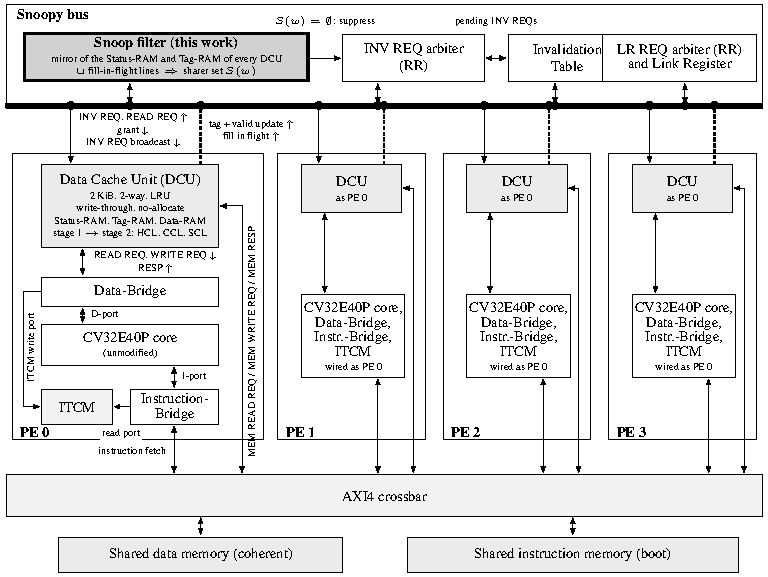
\includegraphics[width=\textwidth]{fig_arch.pdf}
\caption{The system, and what this work adds to it. Four unmodified cores sit
over their private data cache units, which reach shared memory through an AXI4
crossbar and maintain coherence through a single snoopy bus. The snoop filter
holds a mirror of every cache's tag and valid arrays, kept current by one update
port per DCU, and answers the invalidation arbiter's one question: is there
anybody to tell?}
\label{fig:arch}
\end{figure*}

The DCU is a private, write-through, no-allocate L1 data cache sitting between
an in-order RISC-V core and the memory system. Because writes go through to
memory, shared memory always holds the current value and no dirty-line writeback
or ownership state is needed. Coherence is maintained by an invalidation bus:
a core write reaches the bus as an invalidation request, and on grant the
address is broadcast to every other DCU, which drops any matching line.

Two properties of that bus matter here. Plain read requests are not arbitrated
against each other -- multiple readers proceed in the same cycle, which is the
multiple-readers half of the MRSW invariant -- but a read is withheld while
another core has an invalidation outstanding for the same line, which is the
single-writer half. Invalidations \emph{are} arbitrated: at most one is granted
per cycle across the cluster, and the grant is held back until every other DCU
can accept the broadcast, so that no invalidation is ever lost.

Fig.~\ref{fig:arch} shows the system and where the filter sits in it.
Our reproduction targets the stated configuration: four processing elements,
each an unmodified CV32E40P with a private 2\,KiB two-way DCU of 16-byte lines,
meeting shared memories through an AXI4 crossbar. A non-coherent baseline is
built from the same sources with one parameter changed, so any comparison
between them is attributable to the cache sub-system alone.

% =============================================================================
\section{Where the Time Goes}
\label{sec:measure}
% =============================================================================

\subsection{The coherence bus is a large fraction of runtime}

The DCU separates a core access into the places it can wait. One of those is
stage~1 waiting for a snoopy-bus grant. Fig.~\ref{fig:stall} gives that bucket
as a fraction of the cycles a core spent with an access in the DCU at all,
for each kernel at three memory latencies.

\begin{figure}[t]
\centering
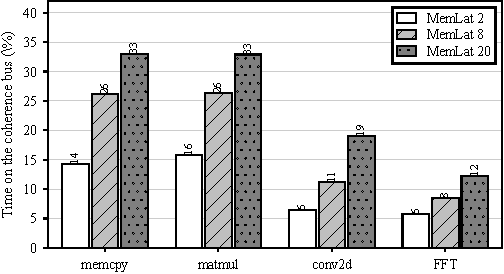
\includegraphics[width=\columnwidth]{fig_stall.pdf}
\caption{Time each core spends waiting for a snoopy-bus grant, as a percentage
of the cycles it had an access in the DCU. Table~\ref{tab:invuse} shows that
none of the traffic it is waiting for is necessary.}
\label{fig:stall}
\end{figure}

Between a twentieth and a third of a core's time goes to arbitrating for a
resource that grants one request per cycle across the whole cluster. The share
grows with memory latency, because each grant is held longer.

\subsection{It is not readers waiting on writers}

The obvious reading of Fig.~\ref{fig:stall} is contention between readers and
writers -- the single-writer screening doing its job. We instrumented the bus to
count it, and across all four kernels a read is \emph{never} withheld: not once.
Whatever the stall is, it is not the MRSW screening.

By elimination it is the invalidations, which are the only arbitrated traffic
left.

\subsection{None of the invalidations are necessary}

Each DCU therefore counts the broadcasts it receives and how many find a line to
clear. Table~\ref{tab:invuse} gives the result.

\begin{table}[t]
\caption{Invalidation broadcasts received across the cluster, and how many
invalidated a line. The last row is a control.}
\label{tab:invuse}
\centering
\begin{tabular}{@{}lrrr@{}}
\toprule
Workload & Broadcasts & Useful & \% \\
\midrule
matmul ($64^2$)      & 823{,}338 & 0 & 0.00 \\
conv2d ($64^2$)      & 139{,}182 & 0 & 0.00 \\
FFT ($N{=}256$)      &  61{,}683 & 0 & 0.00 \\
memcpy (16\,KiB)     &  24{,}618 & 0 & 0.00 \\
\midrule
sharing testbench    &       921 & 345 & 37.46 \\
\bottomrule
\end{tabular}
\end{table}

Over a million broadcasts, none of which invalidated anything. Each one paid a
cluster-wide arbitration and a four-way handshake to inform nobody of anything.

A result this uniform deserves suspicion of the instrument rather than of the
design, so the counter is controlled. Our coherence testbench shares
deliberately, with a producer/consumer ping-pong and a randomised four-core
stress over a small window; on that workload the same counter reports 345 useful
broadcasts of 921. The counter can see a useful invalidation. The zeroes are a
property of the workloads.

They are a property worth stating plainly: these kernels are data-parallel and
partition their data per core, so essentially every written line is private.
That is not a weakness of the benchmark selection, because these are the kernels
the original evaluation itself uses.

% =============================================================================
\section{An Exact Snoop Filter}
\label{sec:filter}
% =============================================================================

\subsection{Structure}

The bus needs to answer one question before granting an invalidation: is there
another cache that has to hear it? A mirror of the caches' tag and valid arrays
answers it, held in the bus and updated by the same two events that change the
caches themselves -- a refill installs a tag into a way, an invalidation clears
one. Each DCU exports those events on a small port driven from the same signals
that write its own arrays.

Exactness is therefore structural rather than argued. The mirror is written from
the same signals, on the same clock edge, under the same conditions as the state
it mirrors, so it cannot drift from it.

We rejected a hashed filter deliberately. A Bloom-style structure may only ever
over-approximate: claiming a line is held when it is not costs a redundant
broadcast and is safe, while the converse loses an invalidation and breaks
coherence. Insert-only hashed filters are safe but saturate, and matmul touches
far more lines than an affordable bitmap has bits; removing from one requires
knowing when a line leaves a cache, which is exactly the information a mirror
already has.

\subsection{Exact about the wrong property}
\label{sec:fill}

A mirror of the tag arrays is exact about which lines each cache \emph{holds},
and that turns out not to be the property the bus needs. A DCU between issuing
its memory read and refilling the victim way holds nothing for the line it is
fetching, so it does not appear in the mirror -- and it is precisely the cache
that must receive the invalidation, because receiving one in that window is what
cancels its refill. Suppress the broadcast and it installs a line that was
invalidated while in flight.

The property is residency \emph{or imminent residency}. Each DCU therefore
exports its refill window alongside its mirror updates, and the filter answers
over the union. The window opens when the cache issues the fetch and closes on
the cycle the refill lands, which is the same cycle the mirror learns the tag:
the two halves abut exactly, so the line is covered in every cycle by one or the
other.

This is not a defensive addition. Counting the granted invalidations for which
no other cache held the line but one was fetching it -- each one a broadcast a
committed-tag mirror would have wrongly suppressed -- our coherence testbench
reports 20 of 2{,}241 over ten randomised interleavings, and at least one in
every one of the ten. The window is narrow enough that the design passed 3{,}139
checks before the counter existed, which is how a race of this shape usually
survives a test suite.

\subsection{Why suppression is safe}

When the answer is that no other cache holds the line or is fetching it, a
broadcast could clear nothing anywhere, and not sending it is unobservable. That
is the whole argument, and it is short because the structure is exact. A
conservative filter would need an argument about the direction of its error;
this one needs only that it asks about the right state.

Everything else is untouched. Invalidations that \emph{are} needed are still
arbitrated, broadcast and acknowledged exactly as before; the single-writer
screening on reads is unchanged; and the write-through lock that stops a remote
read fetching a pre-write value is unchanged, because it protects against a
value in memory rather than against a cached copy.

\subsection{Implementation}

The mirror is one array per (core, way) pair, each with a single write port and
a single read port, addressed by set index -- eight arrays at the geometry
studied here. Tags are held outside any reset, since a tag is only compared when
its valid bit says it means something, which lets them map to distributed RAM.
Valid bits stay in flip-flops, where they can be reset and read eight at a time,
at 512 bits rather than 11{,}264. This is the same division the DCU makes
internally for the same reason.

That structure matters more than it might appear: a first implementation held
tags and valid bits together under an asynchronous reset and read them
combinationally, which Vivado mapped entirely to flip-flops -- 11{,}776 of them,
and 3{,}202 LUTs, against 512 and 408 for the structure above.

% =============================================================================
\section{Evaluation}
\label{sec:eval}
% =============================================================================

\subsection{Cycles}

\begin{figure*}[t]
\centering
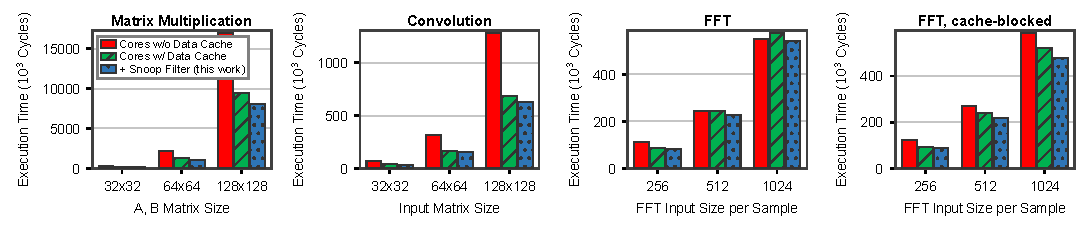
\includegraphics[width=\textwidth]{fig_exec.pdf}
\caption{Execution time of the three benchmark kernels against problem size,
without a data cache, with one, and with the snoop filter of this work. The
axes are those of the original's own execution-time figure, so the first two
bars of each cluster are directly comparable with it. Matrix multiplication and
convolution reproduce the reduction it reports; FFT does not, and the reason is
capacity rather than coherence -- see the text.}
\label{fig:exec}
\end{figure*}

Fig.~\ref{fig:exec} places the extension on the original's own axes: execution
time per kernel against problem size, uncached against cached, with our filter
added as a third bar the original has no counterpart to.

Two of the three reproduce it: matrix multiplication by 38.4 to 44.0\% and
convolution by 46 to 48\%, against the ${\approx}40\%$ the original reports for
both. Neither decays with problem size, and that is not luck. What must stay resident is not the data set but the \emph{reuse
footprint}, the bytes a core revisits before moving on -- one row of $B$ for
matrix multiplication, $4N$ bytes or 512\,B at $N{=}128$, and the three-row
sliding window for convolution, $12N$ bytes or 1536\,B. Both fit a 2\,KiB DCU
throughout, so the benefit does not move.

FFT is where that stops holding. The original reports a uniform
${\approx}23\%$; we match it at $N{=}256$, at 24.8\%, but the benefit falls to
0.4\% at 512 and turns negative at 1024, where the cache makes the kernel
\emph{slower} than having none. The footprint argument predicts exactly this:
FFT revisits $N$ complex points across its stages, $8N$ bytes, which is 2\,KiB
at $N{=}256$ and 8\,KiB at $N{=}1024$. Only the first fits.

That the cause is capacity and not conflict can be shown rather than asserted,
by moving one variable at a time. At $N{=}512$, doubling associativity at the
same 2\,KiB recovers 3.8\%; quadrupling capacity at the same associativity
recovers 24.5\%, and 16\,KiB recovers nothing beyond 8\,KiB. Saturation once the
footprint fits is the signature of a capacity limit, not a conflict one. Given a
DCU that holds the footprint, FFT then reproduces the original at every size --
24.8, 24.8 and 24.5\% at 8\,KiB. At the 2\,KiB its text states, it does not. We
read that as a configuration discrepancy rather than a contradiction: its result
implies a cache larger than the one specified, or a smaller working set, and the
published description does not let a reader tell which.

None of it weakens the filter, which is orthogonal: the filter removes coherence
traffic, not misses. It is worth roughly 50\% throughout on the first two
kernels, and at $N{=}1024$ it is what carries FFT back from $-4.3\%$ to parity.

%% The per-kernel speedup table was folded into the paragraph below. Three of
%% its four rows duplicated bars now in Fig. \ref{fig:exec}; what it uniquely
%% carried -- memcpy, and the oracle column -- is two sentences, and the page
%% limit was worth more than the fourth restatement of the same four numbers.

Against the unfiltered design the filter is worth $1.222\times$ on matrix
multiplication, $1.123\times$ on memcpy, $1.089\times$ on convolution and
$1.061\times$ on FFT: a geometric mean of $1.122\times$. The useful comparison
is not that mean but an oracle that suppresses every broadcast unconditionally,
which is sound to simulate only because Table~\ref{tab:invuse} says none are
needed, and which bounds what any filter could return.

%% fig_result removed to make room for fig_exec, which supersedes it: its panel
%% (a) plotted what the extension is worth against no cache, which fig_exec now
%% does for three kernels at three sizes rather than one size each. Its panel
%% (b), the snoop-stall reduction, survives as the numbers in the paragraph
%% below -- conv2d 20,848 to 109, memcpy 7,168 to 1 -- so no evidence is lost
%% with it. paper/fig_result.pdf is still generated by scripts/plot_date.py if
%% a venue with a looser page limit wants it back.

The filter reaches the oracle on every kernel, cycle for cycle. That is what an
exact structure should do on workloads with no sharing: it suppresses precisely
the broadcasts the oracle does, for a provable reason rather than an assumed
one.

The snoop-stall bucket confirms the mechanism rather than merely the outcome.
On conv2d it falls from 20{,}848 cycles to 109; on memcpy, from 7{,}168 to 1.
FFT is the exception and falls only from 6{,}521 to 2{,}955, because
load-reserved and store-conditional still pass the second arbiter whatever the
broadcasts do -- a residual cost no filter can remove.

\subsection{The extension stops being harmful}

The reproduction's most awkward finding was that on memcpy at low memory
latency, the cache extension is \emph{slower} than having no cache at all:
$0.975\times$ the non-coherent baseline. With the filter it runs at
$1.095\times$. The pathology is not intrinsic to attaching a coherent cache; it
is the cost of announcing private writes to a cluster that does not care.

\subsection{Coherence}

The four kernels never exercise the filter's must-broadcast path, so they cannot
establish that it is safe. Our coherence testbench does: it shares deliberately,
and roughly half of its invalidations are useful. With the filter enabled it
passes 3{,}112 checks, including a version-monotonicity invariant -- a core that
has observed version $k$ of a location may never afterwards observe a version
below $k$, which is exactly what a lost invalidation causes -- and a final
quiesce in which every core re-reads the whole window so that any line left
stale in any cache is caught against memory. The filter suppressed 282 of 921
broadcasts and delivered every one that mattered.

\subsection{FPGA cost}

Both configurations were implemented on a Zynq UltraScale+ XCZU7EV in a
non-project Vivado 2025.1 flow.

%% Per-module resource breakdown. Generated from
%%   python scripts/table1.py filtered
%% and transcribed here; regenerate that if the build changes.
%%
%% Single column, in the shape of the original's Table I: the module tree down
%% the left, then LUTs, FFs, BRAMs, DSPs, and Available / Utilisation rows
%% under the rule. The instance count is folded into the name and the LUTRAM
%% column is gone -- the one number from it that matters, the filter's 208
%% LUTRAM out of 408, is stated in the text where it is argued.
%%
%% Re-measured 2026-09-08 against the RTL that covers fills in flight, both
%% variants in one batch. No total row inside the tree on purpose: Vivado's
%% figure for the SoC is not the sum of the rows above it -- a LUT shared across
%% a hierarchy boundary counts against both children but once against the
%% parent -- so a total under the column would read as an arithmetic error. The
%% tool's own figures sit below the rule instead, where they are plainly a
%% separate statement.
\begin{table}[t]
\caption{Post-implementation resources, XCZU7EV at 60\,MHz, filtered build.
Sub-rows may sum slightly above their parent, because a LUT shared across a
hierarchy boundary is counted against both children but only once against the
parent. The figures below the rule are the tool's own, not column sums.}
\label{tab:fpga}
\centering
\footnotesize
\setlength{\tabcolsep}{3.5pt}
\begin{tabular}{@{}lrrrr@{}}
\toprule
Module & LUTs & FFs & BRAMs & DSPs \\
\midrule
\textbf{Processing element} ($\times$4)      & 17{,}833 & 9{,}948 & 32 & 20 \\
\quad RISC-V core, CV32E40P                  & 16{,}929 & 8{,}404 &  0 & 20 \\
\quad ITCM + Instr.-Bridge                   &      252 &      36 & 32 &  0 \\
\quad Data-Bridge                            &      319 &      32 &  0 &  0 \\
\quad AXI4 masters ($\times$3 per PE)        &      333 & 1{,}476 &  0 &  0 \\
\addlinespace[2pt]
\textbf{Cache extension}                     & \textbf{6{,}540} & \textbf{4{,}628} & 20 & 0 \\
\quad Data Cache Unit ($\times$4)            & 5{,}816 & 3{,}998 & 20 &  0 \\
\quad\quad controller + HCL                  & 2{,}860 & 2{,}846 &  0 &  0 \\
\quad\quad tag RAM                           & 1{,}677 &      96 &  4 &  0 \\
\quad\quad data RAM                          & 1{,}289 & 1{,}056 & 16 &  0 \\
\quad Snoopy bus                             &      728 &     630 &  0 &  0 \\
\quad\quad round-robin arbiter               &      251 &       2 &  0 &  0 \\
\quad\quad Invalidation Table                &       69 &     116 &  0 &  0 \\
\quad\quad \textbf{snoop filter (this work)} & \textbf{408} & \textbf{512} & 0 & 0 \\
\addlinespace[2pt]
\textbf{AXI4 crossbar}                       & 2{,}125 &     279 &  0 &  0 \\
\textbf{Shared data memory}, 256\,KiB        &      724 &     150 & 64 &  0 \\
\textbf{Shared instr.\ memory}, 32\,KiB      &      506 &      86 &  8 &  0 \\
\textbf{Control region}                      &      113 &     259 &  0 &  0 \\
\midrule
Whole device, as reported by the tool        & 27{,}845 & 15{,}670 & 124 & 20 \\
\addlinespace[1pt]
Available                                    & 230{,}400 & 460{,}800 & 312 & 1{,}728 \\
Utilisation (\%)                             &    12.09 &     3.40 & 39.74 & 1.16 \\
\bottomrule
\end{tabular}
\end{table}


Table~\ref{tab:fpga} gives the breakdown. The filter costs 1{,}064 LUTs and
516 flip-flops over the unfiltered design, under 4\% of it, and no block RAM or
DSP at all. Both configurations meet every constraint with no failing endpoints,
at $+1.199$~ns and $+1.265$~ns of slack respectively -- so at this operating
point the filter costs essentially no slack, 66~ps on a 16.667~ns period.

Both figures come from one source tree with one parameter changed, implemented
in the same batch, which is the only way a slack comparison on this design means
anything: an earlier pair of runs weeks apart put the same two configurations at
$+4.307$ and $+2.597$~ns, a 1.7~ns spread in the opposite direction, from
netlists differing by fourteen LUTs. Place-and-route outcomes move by more than
the effect being measured, so we quote slack only within a batch and never
across one.

Two things in the breakdown are worth drawing out. Half of the filter's 408
LUTs are distributed RAM holding the mirror, and its 512 flip-flops are exactly
the valid bits, four cores by 64 sets by two ways: the structure went in as
intended, with tags in memory and only the resettable state in registers. And
within the DCU the controller outweighs the storage, 2{,}802 LUTs against
1{,}677 for the tag array and 1{,}285 for the data array, because at 2\,KiB the
arrays are nearly free and the coherence logic is not.

\subsection{The frequency it costs}

It does cost frequency, and the paper would be misleading without saying so. At
a 75~MHz target the reference meets timing with $+1.327$~ns of slack and the
filtered design does not, at $-2.586$~ns. The critical path is 86\% routing and
runs from a DCU's registered request address across the die; the filter
lengthens it because the decision to broadcast is a cluster-spanning
combinational path, and it does so however the mirror is built. Making the
mirror smaller did not help: the flip-flop version above is four times the area
and closes \emph{better}, at $-0.423$~ns.

We therefore evaluate at 60~MHz, which both configurations meet comfortably, and
which is the frequency the original design itself runs at rather than one chosen
for convenience. At a fixed 60~MHz clock the filter's $1.122\times$ in cycles is
a $1.122\times$ in wall time. Clocked freely, the reference reaches a higher
frequency and the advantage narrows.

We deliberately do not report a maximum-frequency comparison from the 60~MHz
builds. Measured at a constraint that is already met, that figure records where
the tool stopped optimising rather than what the design can do: at 60~MHz it
favours the filtered design by 9.8~MHz, and at 75~MHz it favours the reference
by 20.5~MHz.

% =============================================================================
\section{What Did Not Work}
\label{sec:rejected}
% =============================================================================

Three mechanisms preceded this one. We report them because each was rejected by
a measurement that also sharpened the eventual design.

\textbf{A streaming mode} that would skip allocation and read at word
granularity for phases with no reuse. The non-coherent baseline already is such
a mode, and bounds it: on memcpy it beats the cache at a memory latency of two
by 2.5\% and loses by better than two to one at eight and twenty, because a line
fill amortises one memory latency across four words.

\textbf{A hit-speculative bypass}, in which a read presumes it will hit and
takes no bus transaction, and only a miss arbitrates. It was both useless and
incorrect. Useless because plain reads were never arbitrated in the first place,
so there was no cost to remove -- it measured slower. Incorrect because the
screening it removed is not about allocation but is the single-writer half of
MRSW: a read that hits a resident line while a remote invalidation for that line
is outstanding returns stale data. It passed all eleven functional checks of the
benchmark harness, which is the point worth reporting: the race window is narrow
and a green test said nothing about it.

\textbf{Two structural fixes to the mirror}, described in
Section~\ref{sec:eval}: neither the register count nor the storage type was the
cause of the frequency loss.

\textbf{Directed invalidation}, the obvious next step, which does not pay. The
mirror knows not merely \emph{whether} another cache holds the line but
\emph{which} ones do, so the bus can invalidate exactly those and hold the grant
on only those: an exact multicast with a partial barrier. Only an exact filter
may do this, since under multicast a missing sharer bit loses an invalidation
rather than costing a redundant broadcast. Measured on a halo-exchange stencil
whose band boundaries give a sharer set of exactly one of three, it behaves
perfectly -- 168 invalidations delivered, all 168 useful, against suppression's
504, with the residual stall down elevenfold -- and is worth 0.1 to 0.3\% at
every memory latency tried. Exact suppression has already removed the traffic
that caused the serialisation, and the remainder is irreducible: somebody does
have to be told, and the writer does have to wait. Once the filter is exact, the
residue is not worth steering.

% =============================================================================
\section{Threats to Validity}
% =============================================================================

The central measurement is that none of the invalidation traffic is useful, and
that is a property of workloads as much as of the design. Data-parallel kernels
that partition per core have almost nothing to share. We claim only what we
measured: on the kernels the original evaluation itself uses, this design's
coherence traffic is entirely avoidable. The halo-exchange stencil of
Section~\ref{sec:rejected} is the case with genuine sharing, and the filter is
still worth $1.11\times$ there at a memory latency of twenty, because the
interior of each band is private even when its boundary is not. Our coherence
testbench, at roughly half its invalidations useful, is the extreme in the other
direction.

The evaluation is in cycles from RTL simulation and in post-place-and-route
resource and timing figures; no bitstream has been run on hardware. The original
targets a Virtex UltraScale+ XCVU9P and this work an XCZU7EV, so absolute
figures are directional rather than a like-for-like comparison.

Power is not reported: Vivado's vectorless estimate models this design as idle,
because it cannot evaluate the cores' clock-gate enables.

% =============================================================================
\section{Conclusion}
% =============================================================================

A seamless coherent cache extension for soft RISC-V multicores spends between 6
and 33\% of each core's time on a coherence protocol that, on its own benchmark
kernels, accomplishes nothing: over a million invalidation broadcasts, none of
which invalidate anything. An exact mirror of the caches' tag arrays lets the
bus suppress those broadcasts for 1{,}064 LUTs and 516 flip-flops, preserving
coherence structurally rather than by argument, and is worth a geometric mean
$1.122\times$ at a fixed 60~MHz clock. It also removes the case in which the
extension was slower than having no cache at all. The mechanism costs
frequency, and we report where that matters.

\ifanon
\else
The design, the measurements and the scripts that regenerate every table are
available at \url{https://github.com/Krishna-Gorai/riscv-cache-extension}.
\fi

\begin{thebibliography}{1}
\bibitem{kamaleldin2024}
A.~Kamaleldin, M.~Nickel, S.~Wu and D.~G\"ohringer,
``Seamless Cache Extension for FPGA-based Multi-Core RISC-V SoC,''
in \emph{Proc. IEEE 37th Int. System-on-Chip Conf. (SOCC)}, 2024.

\bibitem{jetty}
A.~Moshovos, G.~Memik, B.~Falsafi and A.~Choudhary,
``JETTY: Filtering Snoops for Reduced Energy Consumption in SMP Servers,''
in \emph{Proc. 7th Int. Symp. High-Performance Computer Architecture (HPCA)},
2001.

\bibitem{cgct}
J.~F.~Cantin, M.~H.~Lipasti and J.~E.~Smith,
``Improving Multiprocessor Performance with Coarse-Grain Coherence Tracking,''
in \emph{Proc. 32nd Int. Symp. Computer Architecture (ISCA)}, 2005, pp.
246--257.

\bibitem{regionscout}
A.~Moshovos,
``RegionScout: Exploiting Coarse Grain Sharing in Snoop-Based Coherence,''
in \emph{Proc. 32nd Int. Symp. Computer Architecture (ISCA)}, 2005, pp.
234--245.

\bibitem{tilelink}
W.~Terpstra,
``TileLink: A Free and Open-Source, High-Performance Scalable Cache-Coherent
Fabric Designed for RISC-V,'' in \emph{RISC-V Workshop}, 2017.

\bibitem{openpiton}
J.~Balkind \emph{et al.},
``OpenPiton+Ariane: The First Open-Source, SMP Linux-booting RISC-V System
Scaling from One to Many Cores,'' in \emph{Workshop on Computer Architecture
Research with RISC-V (CARRV)}, 2019.

\bibitem{cifer}
A.~Li \emph{et al.},
``CIFER: A Cache-Coherent 12nm 16mm$^2$ SoC with Four 64-Bit RISC-V Application
Cores, 18 32-Bit RISC-V Compute Cores, and a 1541 LUT6/mm$^2$ Synthesizable
eFPGA,'' in \emph{IEEE Int. Solid-State Circuits Conf. (ISSCC)}, 2023.
\end{thebibliography}

\end{document}
